% THIS IS SIGPROC-SP.TEX - VERSION 3.1
% WORKS WITH V3.2SP OF ACM_PROC_ARTICLE-SP.CLS
% APRIL 2009
%
% It is an example file showing how to use the 'acm_proc_article-sp.cls' V3.2SP
% LaTeX2e document class file for Conference Proceedings submissions.
% 

\documentclass{acm_proc_article-sp} 

\usepackage{fainekos-macros}
\usepackage{color}
\usepackage[english]{babel}
\usepackage{acronym}
\usepackage{url}
\usepackage[ruled]{algorithm}
\usepackage{algpseudocode}
\usepackage{paralist}
\usepackage{ragged2e}
\setboolean{HIGHLIGHTCHANGES}{FALSE}
%\setlength{\bibspacing}{\baselineskip}
%\usepackage[tight,footnotesize]{subfigure}

\newcommand{\tikzcircle}[2][black,fill=black]{\tikz[baseline=-0.5ex]\draw[#1,radius=#2] (0,0) circle ;}
\newcommand{\slabel}{\sigma}
\newcommand{\tlabel}{\slabel_\chi}
\newcommand{\ulabel}{\slabel_u}
\newcommand{\labelSet}{\Sigma}
\newcommand{\ulabelSet}{\labelSet_u}
\newcommand{\bslabel}{\bar{\slabel}}
\newcommand{\tlabelSet}{\labelSet_\chi}
\newcommand{\btlabel}{\bar{\tlabel}}
\newcommand{\trans}[1]{\xrightarrow{#1}}
\newcommand{\out}[1]{\left\langle #1\right\rangle}
\newcommand{\Omapeps}{\Oc_\varepsilon}
\newcommand{\hsOut}{f}
\newcommand{\CDtau}{\textbf{CD}_\tau(\Sys_1 , \Sys_2)}
\newcommand{\simu}{\mathcal{S}}
\newcommand{\bisimu}{\mathcal{B}}
\newcommand{\Ft}{\Fc_t}
\newcommand{\Fd}{\Fc_d}
\newcommand{\partition}{\mathcal{P}}
\newcommand{\SHS}{\Sigma}
\newcommand{\simue}{\simu^\varepsilon}
\newcommand{\hx}{\hat{\stPt}}
\newcommand{\Cc}{\mathcal{C}}
\newcommand{\egm}{s}
\acrodef{NSR}{Normal Sinus Rhythm}
\acrodef{AP}{Action Potential}
\acrodef{ICD}{Implantable Cardioverter Defibrillator}
\acrodef{SVT}{SupraVentricular Tachycardia}
\acrodef{VT}{Ventricular Tachycardia}
\acrodef{VF}{Ventricular Fibrillation}
\acrodef{SVT}{SupraVentricular Tachycardia}
\acrodef{EGM}{electrogram}
\acrodef{CA}{cellular automata}

\newboolean{REPORT}
\setboolean{REPORT}{FALSE}
\linespread{0.97}

\begin{document}

\title{Model Checking Implantable Cardioverter Defibrillators}

\author{
% 1st. author
\alignauthor
Houssam Abbas, Kuk Jin Jang, Zhihao Jiang, Rahul Mangharam\\
       \affaddr{Department of Electrical and Systems Engineering}\\
       \affaddr{University of Pennsylvania, Philadelphia, PA, USA}\\
       \email{\{habbas,  jangkj, zhihaoj, rahulm\}@seas.upenn.edu}
}
% Just remember to make sure that the TOTAL number of authors
% is the number that will appear on the first page PLUS the
% number that will appear in the \additionalauthors section.

\maketitle
\begin{abstract}
Ventricular Fibrillation is a disorganized electrical excitation of the heart that results in inadequate blood flow to the body.
It usually ends in death within seconds.
The most common way to treat the symptoms of fibrillation is to implant a medical device, known as an \emph{Implantable Cardioverter Defibrillator} (ICD), in the patient's body.
Model-based verification can supply rigorous proofs of safety and efficacy. 
In this paper, we build a hybrid system model of the human heart+ICD closed loop, and show it to be a \yhl{STORMED system, a class of o-minimal hybrid systems that admit finite bisimulations.}
In general, it may not be possible to compute the bisimulation.
We show that approximate reachability can yield a finite \emph{simulation} for STORMED systems, which improves on the existing verification procedure.
In the process, we show that certain compositions respect the STORMED property.
Thus it is possible to model check important formal properties of ICDs in a closed loop with the heart, such as delayed therapy, missed therapy, or inappropriately administered therapy. 
The results of this paper are theoretical \yhl{and motivate the creation of concrete model checking procedures for STORMED systems.}
\end{abstract}

%Ventricular Fibrillation is a disorganized electrical excitation of the heart that results in inadequate blood flow to the body.
%It usually ends in death within a few seconds.
%The most common way to treat the symptoms of fibrillation is to implant a medical device, known as an Implantable Cardioverter Defibrillator (ICD), in the patient's body.
%Model-based verification can play a crucial role in ICD development.
%In this paper, we build a hybrid system model of the human heart+ICD closed-loop system, and show that it admits a finite bisimulation by showing it to be a STORMED hybrid system.
%In general, it may not be possible to compute the bisimulation.
%We show that approximate reachability can yield a finite \emph{simulation} for STORMED systems, which improves on the existing verification procedure.
%In the process, we show that certain compositions respect the STORMED property.
%Thus it is possible to model check important formal properties of ICDs in a closed loop with the heart, such as delayed therapy, missed therapy, or inappropriately administered therapy. 
%The results of this paper are theoretical, since no model checkers exist for STORMED systems. 
%In future work we will implement a procedure for model checking the heart+ICD loop.
%% A category with the (minimum) three required fields
%\category{H.5.1}{Computing methodologies}{Modeling and simulation}[Model development and analysis]
%%A category including the fourth, optional field follows...
%\category{L.2}{Applied computing}{Life and medical sciences}
%\terms{Medical devices, life-critical CPS, STORMED systems, heart modeling, ICDs}

\section{Introduction}
\label{introduction}

%\todo[inline]{stress the timing aspect more}
Implantable medical devices such as pacemakers are designed to improve physiological conditions with very little human intervention. 
Their ability to autonomously affect the physiological state of the patient makes the medical devices safety-critical, and sufficient evidence for their safety and efficacy should be provided before the devices can be implanted in the patients. Medical devices increasingly rely on software, and device function and their clinical performance can be affected by seemingly minor changes to software.
%As more functionality is added to the devices
\footnote{In what follows, the word `device' is used to refer to the software of the device.}
%, the complexity of the software component of the device is increasing dramatically, leading to a large number of potential safety violations because of software bugs. 

Over the course of the past four decades, cardiac rhythm management devices such as pacemakers and implantable cardioverter defibrillators (ICD) have grown in complexity and now have more than 80,000 to 100,000 lines of software code~\cite{pauljones}. In 1996, 10\% of \emph{all} medical device recalls were caused by software-related issues and this rose to 15\% between 2003-2012~\cite{recall_stats,killedbycode}. There is currently no standard for testing, validating, and verifying the software for implantable medical devices~\cite{fda1,fda3}.

There are two categories of device bugs: 
1) the device may fail to conform to its \emph{specifications}, that is, the prescription of how it should react to certain inputs.  
2) the device may fail to improve the conditions of the patient as promised, even if it conforms to its specifications. 
The desired physiological conditions that the closed-loop system should achieve are captured in the \emph{physiological requirements}; for example, for a pacemaker, the heart rate should always be maintained above a certain threshold. 
%In what follows, the word `requirement' always refers to such physiological requirements.
%Note that requirements are about \emph{the closed-loop system}: they prescribe the behavior of both device and environment (e.g. both pacemaker and heart).

Bugs in the first category (non-conformance to specification) can be detected via systematic and extensive open-loop testing in which a set of input sequences is fed to the device, and its output is compared with the expected output.
Bugs in the second category (violation of physiological requirements), on the other hand, require the availability of the \emph{closed-loop system}, which consists of the device and its environment.
For instance, the pacemaker and the heart as its environment. 
In the medical device industry, closed-loop verification of the physiological requirements is mostly performed in terms of clinical trials, in which the actual devices are implanted in human subjects over an extended duration.
Unfortunately, because of the extremely high cost of clinical trials (several million dollars and spanning several years~\cite{trial_cost}), the amount and variety of human subjects during the clinical trials are limited, which reduces the opportunity to find bugs. 
Moreover, clinical trials are often conducted at the final design stage. Fixing bugs at this stage is very costly.

Closed-loop model checking enables closed-loop evaluation of the physiological requirements at an earlier design stage, which requires formal model(s) of the physiological environment. 
%Depending on the formalism used to model the environment (and device) and the language used to express the requirements, this allows the usage of formal methods to perform the verification.
%Formal environment modeling introduces new challenges that do not arise when modeling the device alone, and this paper aims at addressing these issues in the context of pacemaker verification.
%In the rest of this paper, we speak therefore of pacemaker as the Device Under Verification (DUV) and of the heart as being the environment, but it is understood that the discussion carries more broadly, with possible domain-specific adjustments.
In closed-loop model checking, there is only one device model. 
However there can be a large number of environmental conditions which require different models to represent them. For instance, a heart with atrial flutter has an additional conduction pathway that is not present in a healthy heart, causing fast atrial rate. The timing and structural differences of different heart conditions should be distinguished in corresponding heart models.
%\todo[inline]{should we give an example of a heart condition?}
A set of initial models of the environment can be constructed but the set is inherently incomplete because of the large number of environment conditions and their combinations. 
As a result, performing model checking using every model in the set cannot ensure full coverage of the environmental conditions. 

In this paper, domain-specific over-approximation rules are developed that produce abstract models that not only cover explicitly modeled environment conditions, but also cover timing behaviors and conditions not modeled in the set of initial models. 
The abstract models can be then used for closed-loop model checking of the device model. 
If the closed-loop system satisfies a requirement, the device under verification satisfies the requirement under environment conditions covered by the abstract models. 
However, if the requirement is not satisfied, the model checker returns a counter-example. 
In device modeling, the counter-example is considered \emph{spurious} if it can not be produced by the device (as shown in (\figref{distinction}(a)).
However in environment modeling, even if the counter-example can not be produced by any of the initial environment models, it might still be a physiologically valid behavior.
Thus the validity of a counter-example cannot be determined by refining the environment model, but can ultimately only be determined by domain experts. 

Counter-examples returned from abstract models can be difficult to interpret by domain experts.
One abstract counter-example could be produced by multiple physiologically valid conditions, which causes ambiguity.
Thus, a rigorous framework is necessary to balance the need to cover a wide range of environmental conditions and the need to provide counter-examples to the physicians within their physiological context.

Another challenge for closed-loop model checking of medical devices is the amount of domain expertise needed during: 1) physiological modeling, 2) model abstraction and refinement, and 3) checking the validity of counter-examples.
Thus the framework must also allow non-domain experts to perform verification (item 2 above),
and establish `hand-off' points where the results of verification can be handed back 
to the experts for interpretation.

\begin{figure}[!t]
		\centering
		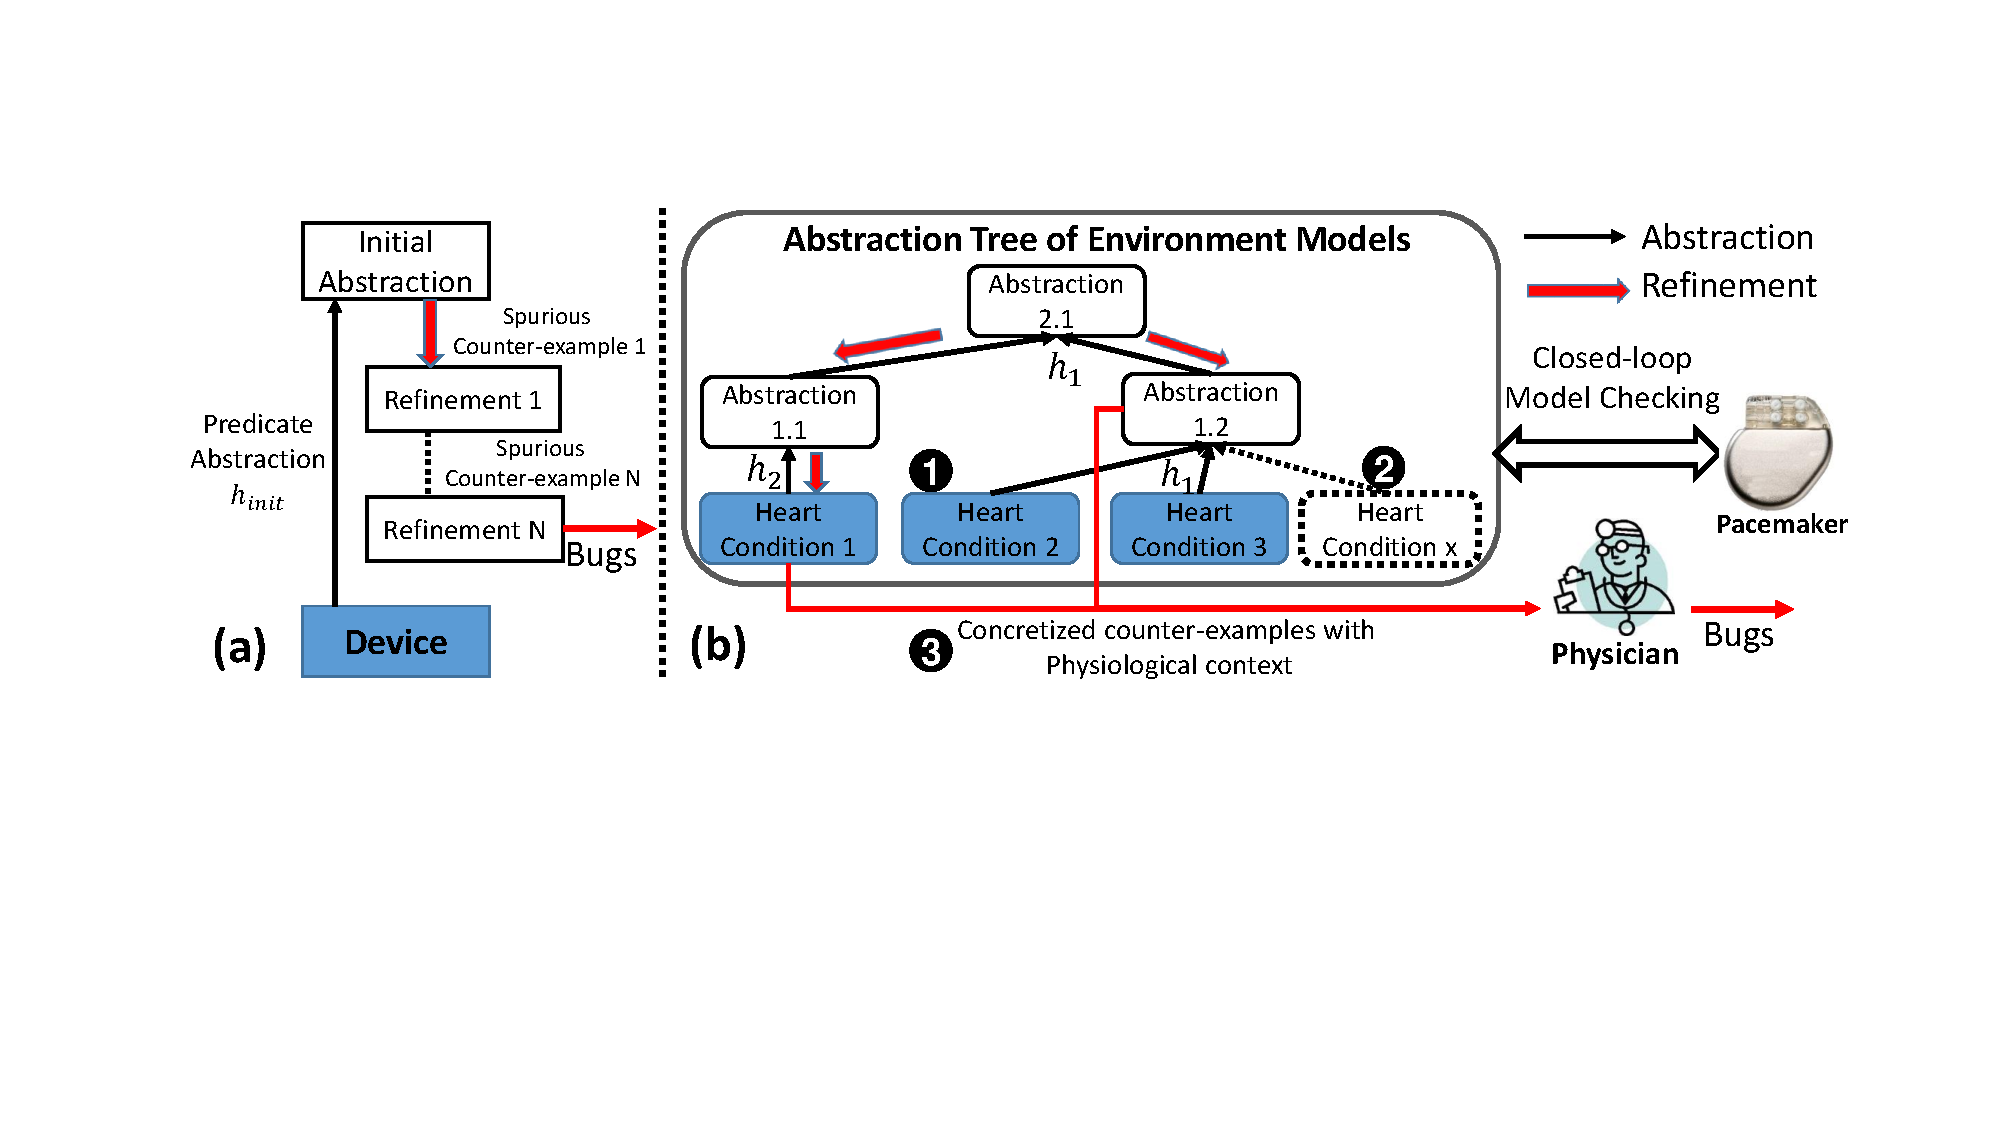
\includegraphics[width=\textwidth]{figs/distinction.pdf}
		%\vspace{-5pt}
		\caption{\small (a) Device modeling with CEGAR framework (b) Closed-loop model checking with environment abstraction tree.}% The initial set of heart conditions are first abstracted and/or merged using abstraction rules $h_1,h_2$ (Marker 1). The abstract model is first used for closed-loop model checking. When a property violation happens, refined models in the abstraction tree are used for model checking. The most concrete counter-examples may be available in the initial model(s) (Marker 2). In the scenario where counter-examples do not exist in explicitly modeled Heart condition 2 and 3, the counter-example in Abstraction 1.2 may correspond to a valid heart condition introduced during abstraction $h_1$. The physician decides the validity of the counter-examples.}
		  \vspace{-10pt}
		\label{fig:distinction}
\end{figure}


\subsection{Contributions}
In this paper a framework is proposed for environment modeling in closed-loop model checking of medical device software.
The cardiac pacemaker is used as an example of applying this framework.
An expandable set of timed-automata heart models are first developed to represent different physiological conditions (\figref{distinction} Marker 1).
A set of domain-specific abstraction rules are then developed based on physiological knowledge, which help ensure the physiological relevance of the behaviors introduced into the abstract models (\figref{distinction} Marker 2).
Then the rules are applied to the initial set of physiological models to obtain an abstraction tree, which will be used for closed-loop model checking of the pacemaker. 
A straightforward search procedure is then used to conduct model checking using suitable heart models and return the most concrete and unambiguous counter-examples to the physicians for analysis (\figref{distinction} Marker 3).
In this framework, physiological knowledge is only needed when constructing the initial model set and when analyzing counter-examples. 
The application of the physiological abstraction rules and the verification procedure can be automated.
The proposed method can potentially be generalized to other domains in which the device operates in a large variety of environmental conditions.
\subsection{Related Work}
%\todo[inline]{complete}
Counter-Example Guided Abstraction Refinement (CEGAR) \cite{CEGAR} has been proposed to over-approximate the behaviors of the device using predicate abstraction (\figref{distinction}.(a)).
%Upon property violation the abstract counter-example is checked for its validity on the actual system. If the counter-example is \emph{spurious} the model is then refined to eliminate the spurious counter-example. 
%This process is then continued on the refined model until either a valid counter-example returns or no counter-examples are returned. 
CEGAR works well during device modeling, however, it cannot be applied to environment modeling for two reasons: 1)~predicate abstraction does not guarantee the validity of behaviors introduced into the model. In fact, for device modeling, all additional behaviors introduced into the abstract model are spurious. 2)~the validity of a counter-example cannot be checked automatically as in device modeling. 

Proof-based approaches have also been applied to verify  abstractions and refinements of pacemaker specification using Event-B~\cite{eventb}. However, the authors did not take into account environment behaviors thus the framework cannot be used for verifying physiological requirements.  

Physiological modeling of cardiac activities has been studied at various levels for different applications. In \cite{natalia}, the electrical activity of the heart is modeled with high spatial fidelity to study the mechanisms of cardiac arrhythmia. In \cite{radu}, formal abstractions of cardiac tissue have been studied to reduce the complexity of the heart tissue model. However, these two models do not focus on the interaction with the pacemaker, therefore cannot be used for closed-loop model checking. In \cite{marta}, hybrid automata models of the heart has been used to capture the complex beat-to-beat dynamics of the heart tissue. However the model cannot be used to cover behaviors across different heart conditions.

In previous work \cite{sttt13} a set of formal heart models covering various heart conditions at different abstraction levels was developed, and closed-loop model checking was performed on models of implantable pacemakers. 
However, the physiological knowledge required during each step of closed-loop model checking prevents the method to be practical.


%During the closed-loop model checking, the most abstract model(s) that are appropriate to the requirement are automatically selected as the initial environment models. If the requirement is satisfied, the system is safe under the environment conditions covered by the initial environment models. If the requirement is violated in certain initial environment model, the children of the model in the abstraction tree are used for model checking until 1) the leaves of the tree is reached, or 2) there is no violations in the child nodes. The counter-examples obtained at the most refined models are returned to the physician for validity check. This process is automated so that no domain knowledge is required for the person who performs model checking. It also ensures the most concrete counter-examples with unambiguous physiological context are returned to the physician for analysis. 
%The first challenge in closed-loop model checking of pacemakers is that the human heart displays a large number of different conditions, henceforth referred to as `physiological conditions'.
%E.g., one heart may display \emph{atrial fibrillation} where the upper chambers of the heart (the atria) produce an exceedingly fast beat that prevents proper blood pumping.
%Another heart may display Premature Ventricular Contraction (PVC) where a location in the ventricles produces electrical impulses at erratic time instants.\Hao{I don't think these two conditions make sense to the reader}
%Each such condition will require its own formal model, and some models may display more than one condition.
%In this paper, we build such a set of formal heart models using the timed automata formalism in Section ???.
%Performing model checking with each model separately, we seek a method that can combine models, and perform model checking on the merged model. 
%The combination of models must be such that if the merged model is correct (according to the requirements) then so is every model that was combined into it.
%We present \emph{abstraction rules} in Section ?? which allow us to do precisely that.

%This initial set of models will necessarily be \emph{incomplete} because the number of physiological conditions is too large, and some of the conditions are too ill-understood for modeling.
%Thus, unlike system modeling in which one typically starts from one ground truth model to be verified, our starting point is an \emph{incomplete set of environment models}.
%Because of this incompleteness, we seek abstraction rules that introduce new \emph{physiologically meaningful} behavior which might actually be produced by heart models not in the initial set.
%These then correspond to heart conditions not taken explicitly into account. 
%This provides a second motivation for the domain-specific abstraction rules $R$ in Section ???, which can be thought of as relaxations of the conditions governing the model's behavior. 
%Like predicate abstraction, they produce models that over-approximate the behavior of the model they are applied to (i.e., $\beh(R(M)) \supset \beh(M)$).
%However, the new behavior they introduce might not be spurious. 
%We demonstrate such a case in Section ???.
%If model checking returns a counter-example on $R(M)$, the physician can decide whether this is actually physiologically plausible behavior and therefore the pacemaker needs to be debugged, or this is indeed spurious and should be thrown out (and the abstraction refined).
%
%Note this is different from classical predicate abstraction [???], which adds behavior in a domain-agnostic fashion. In fact, predicate abstraction is a fist step in the timed automata model checking procedure as presented in [ALur and Dill 1994].
%Our abstraction rules are used to combine and and abstract models \emph{prior} to model checking.
%%tttt
%
%\subsubsection{Contributions}
%In this paper we propose a framework for environment modeling and model checking of medical device software, in particular, pacemakers.
%Specifically, we present several extended timed automata models of various heart conditions in Section ???. 
%We define domain-specific abstraction rules for these models, and demonstrate how these can be applied to gradually add physiologically meaningful behavior in Section ???. 
%Using the models and the rules, we build an abstraction tree which serves to perform model checking of physiological requirements for the heart+pacemaker closed loop in Section ???.
%We illustrate the approach via case studies in Section ???, and conclude in Section ???
%

%

\section{Hybrid systems and simulations}
\label{sec:preliminaries}

This section presents fairly standard definitions on 
%transition systems, 
hybrid systems and their simulations \cite{AlurHLP00ieee}.
It also defines STORMED hybrid systems, which admit finite bisimulations \cite{VladimerouPVD08_STORMED}.

\subsection{Transition and hybrid systems}
\label{sec:transition systems}

%{\large Partitions.} Given a set $Q$, a \emph{partition} $\partition = \{P_1,\ldots,P_k\}$ of $Q$ is a set of disjoint subsets of $Q$ whose union equals $Q$. 
%Let $\equiv_\partition$ be the associated equivalence relation.
%Partition $\partition'$ \emph{refines} $\partition$ if every block $P'$ of $\partition'$ is a subset of some block $P$ of $\partition$; we write this as $\partition' \subset \partition$.
%
\begin{defn}
	\label{defn:transition system}
	A \emph{transition system} $T = (Q,\labelSet,\trans{},Q_0)$ consists of a set of states $Q$, a set of events $\labelSet$ , a transition relation $\trans{} \subset Q \times \labelSet \times Q$, a set of initial states $Q_0$. 
	We write $q \trans{\slabel}q'$ to denote a transition element $(q,\slabel,q') \in \trans{}$.
	Given $P\subset Q$, we define $Post_\slabel(P) \defeq \{q'\;|\;\exists q\in P. q \trans{\slabel}q'\}$
	%
	Given an equivalence relation $\sim$ on $Q$, the \emph{quotient system} $T/\sim$ is
	$T/\sim = (Q/\sim, \{*\}, \trans{}_\sim, Q_0/\sim)$
	where $[q] \trans{*}_\sim [q']$ iff $q \trans{\slabel} q'$ for some $\slabel \in \labelSet$.
	Here $[q]$ is the equivalence class of $q$ and $Q/\sim$ is the set of equivalence classes of $\sim$.
\end{defn}

\begin{defn}
	\label{defn:simulation}	
	Given two transition systems $T_1$ and $T_2$ with the same state space $Q$,
	a \emph{simulation} relation from $T_1$ to $T_2$ is a relation $\simu \subset Q \times Q$ such that 
	for all $(q_1,q_2) \in \simu$, if $q_1 \trans{\slabel}_1 q_1'$, there exists a $q_2' \in Q$ s.t. $q_2 \trans{\slabel}_2 q_2'$ and $(q_1',q_2') \in \simu$.
	A \emph{bisimulation relation} between $T_1$ and $T_2$ is both a simulation relation from $T_1$ to $T_2$ and from $T_2$ to $T_1$.
\end{defn}
%Given a partition $\partition$ of $Q$, the \emph{natural bisimulation} between $T$ and $T/\partition$ is $\Bc_P = \{(q,P) \in Q \times \partition \;|\; q \in P\}$.	
%Conversely, a bisimulation $\Bc$  of $T$ defines a partition $\partition_\Bc$ of $Q$ where $q,q'$ are in the same block of the partition iff $(q,q') \in \Bc$.
%
The bisimulation $\bisimu$ is said to \emph{respect} $\sim$ if $(q,q') \in \bisimu \implies q \sim q'$.
%
The following algorithm, if it terminates, yields a finite bisimulation for $T$ that respects the given equivalence relation~\cite{AlurHLP00ieee}.
Moreover, it is the \emph{coarsest} bisimulation (with respect to inclusion) that respects $\sim$.
\begin{algorithm}[t]
		\caption{Computing a bismimulation respecting $\sim$}
		\label{algo:bisimulation}
		\begin{algorithmic}
			\Require Transition system $T = (Q,\labelSet,\trans{},Q_0)$, equivalence relation $\sim$.
			\State Set $\simu = Q/\sim$			
			\While{$\exists P,P' \in \simu$ and $\slabel \in \labelSet$ s.t. $\emptyset \neq P' \cap Post_\slabel(P) \neq P'$}
				\State Set $\simu = \simu \setminus \{P'\} \cup \{P' \cap Post_\slabel(P) , P' \setminus Post_\slabel(P) \}$
			\EndWhile	
			\State Return $\simu$
		\end{algorithmic}
\end{algorithm}
Given a set of atomic propositions $AP$, if $\sim$ is s.t. $q \sim q'$ iff both states satisfy exactly the same set of atomic propositions, then model checking temporal logic properties can be done on the finite bisimulation instead of the possibly infinite $T$.
%The \emph{coarsest} bisimulation $\bisimu$ that refines a partition $\partition$ is one such that there is no other bisimulation $\bisimu'$ satisfying $\partition_\bisimu \subset \partition_{\bisimu'} \subset \partition$.

%Given a subset $P$ of $Q$, we define its $\slabel$-successor as $Post_\slabel(P) = \{q \in Q | \exists p \in P. q \trans{\slabel} p\}$.
%In other words, $Post_\slabel(P)$ is the set of states forward-reachable from $P$ via the event $\slabel$.


%
%Note that the resulting bisimulation is the \emph{coarsest} bisimulation (i.e., with the least number of blocks in its induced partition) that refines $\partition$.
%\subsection{Hybrid systems}
%\label{sec:hybridSystems}
\begin{defn}
	\label{defn:hybrid system}	
	A \emph{hybrid automaton} is a tuple \[\Sys = (\stSet,\modeSet,\hsSet_0,\{f_\mode\}, Inv,E, \{\reset_{ij}\}_{(i,j)\in E}, \{\guard_{ij}\}_{(i,j)\in E})\] where 
		 $\stSet \subset \Re^n$ is the continuous state space equipped with the Euclidian norm $\|\cdot\|$, 
		$\modeSet \subset \Ne$ is a finite set of modes,
		 $\hsSet_0 \subset \stSet \times \modeSet$ is an initial set,
		 $\{f_\mode\}_{\mode \in \modeSet}$ determine the continuous evolutions with unique solutions,
		 $Inv: \modeSet \rightarrow 2^\stSet$ defines the invariants for every mode,
		 $E \subset \modeSet^2$ is a set of discrete transitions,
		 \yhl{$\guard_{ij} \subset \stSet$ is guard set for the transitions (so $\Sys$ transitions $i \rightarrow j$ when $\stPt \in \guard_{ij}$),
		 $\reset_{ij}: \stSet \rightarrow \stSet$ is an edge-specific reset function.}
		 \\
		 Set $\hsSet = \modeSet\times \stSet$.
		 Given $(\mode,\stPt_0) \in \hsSet$, the \emph{flow} $\theta_{\mode}(;\stPt_0):\Re_+ \rightarrow \Re^n$ is the solution to the IVP $\dot{x}(t) = f_\mode (x(t))$, $\stPt(0)=\stPt_0$.
\end{defn}
%
The associated \emph{transition system} is $T_\Sys = (\hsSet,  E \cup \{\tau\},\trans{},\hsSet_0)$ 
where $\hsSet$ is the state set, $E \cup \{\tau\}$ is the label set for transitions, $\hsSet_0$ is the set of initial states, 
and $\trans{} = (\bigcup_{e \in E} \trans{e}) \cup \trans{\tau}$ 
where $(i,\stPt) \trans{e} (j,y)$ iff $e = (i,j), \stPt \in \guard_{ij}, y = \reset_{ij}(\stPt)$ and $(i,\stPt) \trans{\tau} (j,y)$ iff $i = j$ and there exists 
a flow $\theta_i(\cdot;x)$ of $\Sys$ and $t\geq 0$ s.t. $\theta_i(t;x)=y$ and $\forall t' \leq t$, $\theta_i(t';x) \in Inv(i)$.
%Note that the transition $\trans{\tau}$ abstracts away time, i.e. it doesn't preserve information about the duration of continuous flow.
%For a set $P \subset \hsSet$,$P_{|\stSet}$ denotes its projection onto $\stSet$, 
%and $P_{|\modeSet}$ its projection onto $\modeSet$. 
%\begin{defn}
%	\label{defn:reachability operators}[Reachability]
%	Let $\Sys$ be a hybrid system with hybrid state space $\hsSet$, 	 
%	$I = [0,b) \subset [0,+\infty)$ be a (possibly unbounded) interval, 
%	$t \in I$, 
%	and $\epsilon >0$.
%	The \emph{$\epsilon$-approximate continuous reachability operator}, 
%	$\Rc^{\epsilon}_t : 2^\hsSet \rightarrow 2^\hsSet$ is given by
%	\begin{eqnarray*}
%		\Rc^{\epsilon}_t(P) = \{(i,\stPt) \in \stSet | \exists x_0 \in P_{|\stSet}, t \geq 0. 
%		||\theta_i(t;x_0) - \stPt|| \leq \epsilon\} 
%	\end{eqnarray*}
%	where $P = \{i\}\times W$, $W \subset Inv(i)$.
%	%
%	Define also $\Rc^{\epsilon}_I(P) = \cup_{t\in I} \Rc^{\epsilon}_t(P)$.
%	%
%	The (exact) \emph{discrete reachability operator} is:
%	\begin{eqnarray*}
%	\Rc_{d}(P) &=& \cup_{j: (i,j) \in E} \reset_{ij}(P \cap G_{ij})
%	\end{eqnarray*}
%\end{defn}
%%
%For a hybrid system, $Post_\slabel$ computes the forward reach sets, and is implemented by $\Rc^0_{[0,\infty)}$ and $\Rc_d$. 
Let $\sim$ be an equivalence relation on $\hsSet$ and $\hsSet/\sim$ the corresponding partition.
Let $\Fc_t(\hsSet/\sim)$ be the coarsest bisimulation with respect to $\trans{\tau}$\footnote{I.e., $\Ft$ only considers the continuous transition relation: it is a bisimulation of $T_\Sys^c \defeq (\hsSet/\sim,\{*\},\trans{\tau},\hsSet_0/\sim)$.} 
respecting the partition $\hsSet/\sim$, 
and 
$\Fc_d(\hsSet/\sim) \defeq \{(h_1,h_2)  \;|\; (h_1 \trans{e} h_1') \implies (\exists e' \in E, h_2' \; . h_2 \trans{e'} h_2' \land h_1' \sim h_2') \} \cap \hsSet/\sim$ \cite{VladimerouPVD08_STORMED}.
The iteration 
\begin{eqnarray}
\label{eq:Ft,Fd}
W_0 = \Ft(\hsSet/\sim), \quad\forall i\geq 0,\; W_{i+1} = \Ft(\Fd(W_i))
\end{eqnarray}
computes a bisimulation of $\Sys$.
However it does not necessarily terminate for hybrid systems because the system's reach set might intersect a given block of $\hsSet/\sim$ an infinite number of times (see \cite{LaFerrierePS00_Ominimal} for an example).
The class of systems introduced in the next section has the property that the iteration does terminate for it and returns a finite $\simu$.

Given a set of atomic propositions, if $\sim$ is s.t. $\hsPt \sim \hsPt'$ iff both states satisfy exactly the same atomic propositions, then model checking temporal logic properties can be done on the finite bisimulation instead of the possibly infinite $\Sys$.

\subsection{O-minimality and STORMED systems}
\label{sec:ominimality}
We give a very brief introduction to o-minimal structures.
A more detailed introduction can be found in \cite{LaFerrierePS00_Ominimal}, and an exposition of topology and o-minimality in \cite{VanDerDriesBook}.
We are interested in sets and functions in $\Re^n$ that enjoy certain finiteness properties, called order-minimal sets (o-minimal).
These are defined inside \emph{structures} $\Ac = (\Re,<, +,-,\cdot,\exp,\ldots)$.
The subsets $Y \subset \Re^n$ we are interested in are those that are \emph{definable} using first-order formulas $\formula$: $Y = \{(a_1,\ldots,a_n) \in \Re^n \;|\;  \formula(a_1,\ldots,a_n)\}$.
(First-order formulas use the boolean connectives and the quantifiers $\exists,\forall$).
The atomic propositions from which the formulas are recursively built allow only the operations of the structure $\Ac$ on the real variables and constants, and the relations of $\Ac$ and equality.
For example $2x-3.6y < 3z$ and $x=y$ are valid atomic propositions of the structure $\Lc_\Re=(\Re,<, +,-,\cdot)$, while $cosh(x) < 3z$ is not because $cosh$ is not in the structure.
These structures are already sufficient to describe a set of dynamics rich enough for our purposes and for various classes of linear systems.
%\textbf{Formal definitions}.
A \emph{language} is a set of relations, functions and constants.
E.g. $\Lc_\Re = (<,+,-, \cdot,\Re)$ is the language where the only relation is $<$, the functions are $+,-,\cdot$, and the constants are taken from $\Re$,
and  $\Lc_{exp} = (<,+,-, \cdot,\exp, \Re)$ adds the exponential symbol to it.
Let $\Vc = \{x,y,z,x_1,x_2,\ldots\}$ be a set of variables.
A \emph{term} of a language is either a variable, a constant, or $F(\theta_1,\ldots,\theta_m)$ where $F$ is an $m$-ary function expressible in the language and the $\theta_i$ are terms.
E.g. $2x-3.6y$ is a term of $\Lc_\Re$.
The \emph{atomic formulas} of the language are of the form $\theta_1=\theta_2$ or $R(\theta_1,\ldots,\theta_m)$ where $R$ is an $m$-ary relation on the terms $\theta_i$.
E.g., $2x-3.6y < z\cdot z$ is a an atomic formula in $\Lc_\Re$ which uses the terms $2x-3.5y$ and $z \cdot z$.
The set of (first-order) \emph{formulas} is defined recursively as follows: every atomic formula is a formula, and if $\formula_1,\formula_2$ are formulas, then so are $\formula_1 \land \formula_2, \neg \formula_1, \forall x: \formula_1, \exists x:\formula_1$.
Here the symbols are the usual boolean connectives ( conjunction $\land$ and negation $\neg$), and quantifiers (there exists $\exists$ and for all $\forall$).
A \emph{sentence} in the language is a formula where all variables are inside the scope of a quantifier, e.g. $\exists y . (x+y>3)$ is not a sentence.

So far, a language has been defined in a purely syntactic manner.
A \emph{model} of a language is a set $S$ along with an interpretation of the relations, functions and constants of the language.
We are interested in this paper in the model of $\Lc_{exp}$ where the set $S = \Re$, and the symbols $<,+,-, \cdot,exp$ have their usual meaning (less than, addition, etc).
A set $Y \subset \Re^n$ is \emph{definable} in $\Lc_\Re$ if there exists a formula of the model such that $Y$ can be expressed as $Y = \{(a_1,\ldots,a_n) \in \Re^n \;|\; \formula(x_1,\ldots,a_n)\}$.
E.g., the formula $x^2-1=0$ defines the set $\{-1,+1\}$.
Finally, a \emph{theory} is a subset of sentences in the model $\Lc_\Re$, i.e. it is a collection of sentences that are true in $\Lc_\Re$.
\begin{defn}
	\label{defn:ominimal struct}	
	A theory of $(\Re,\ldots)$ is \emph{o-minimal} if the only definable subsets of $\Re$ are finite unions of points and (possibly unbounded) intervals.	
	A function $f:x \mapsto f(x)$ is o-minimal if its graph $\{(x,y) \;|\; y=f(x)\}$ is a definable set.
\end{defn}
We use the terms o-minimal and definable interchangeably, and they refer to the structure $\Lc_{\exp}= (\Re,<, +,-,\cdot,\exp)$, which is known to be o-minimal.
%
The dot product between $x,y\in \Re^n$ is denoted $x \cdot y$, and $d(Y,S)$ is the minimum distance between sets $Y$ and $S$.
\begin{defn}\cite{VladimerouPVD08_STORMED}.
	\label{defn:stormed system}	
	A \emph{STORMED hybrid system} (SHS) $\SHS$ is a tuple $(\Sys,\Ac, \phi,b_-,b_+, d_{min}, \epsilon,\zeta)$ where $\Sys$ is a hybrid automaton, $\Ac$ is an o-minimal structure, $d_{min}, \zeta \in \Re_+$, $b_-,b_+ \in \Re$ and $\phi \in \stSet^n$ such that:
	\\
	\textbf{(S)} The system is $d_{min}$-separable, meaning that for any $e=(\mode, \mode ')\in E$ and $\mode ''\neq \mode'$,$d(\reset_e(\guard_{(\mode ,\mode ')}), \guard_{(\mode' ,\mode '')})>d_{min}$
	\footnote{We updated the definition of separability from \cite{VladimerouPVD08_STORMED} to accurately capture the requirement that if $\Sys$ flows, it flows a uniform minimum distance along $\phi$. For this we need the starting point in the new mode, and any guard out of the mode, to be separated by at least $d_{min}$.}
%	for any two distinct edges $(\mode, \mode'), (\mode ,\mode '')$ in $E$, $\min\{||x_1 - x^2|| \;|\; x_1 \in G_{\mode, \mode'}, x_2 \in G_{\mode ,\mode ''}\} > d_{min}$
	\\
	\textbf{(T)} The flows (i.e., the solutions of the ODEs) are Time-Independent with the Semi-Group property (TISG), meaning that for any $\mode \in \modeSet, \stPt \in \stSet$, the flow $\theta_\mode$ starting at $(\mode , x)$ satisfies: 1) $\theta_{\mode}(0;x) = x$, 2) for every $t,t' \geq 0$, $\theta_{\mode}(t+t';x) = \theta_{\mode}(t'; \theta_\mode(t;x))$
	\\
	\textbf{(O)} All the sets and functions of $\Sys$ are definable in the o-minimal structure $\Ac$
	\\
	\textbf{(RM)} The resets and flows are monotonic with respect to the same vector $\phi$, meaning that \\
	1) (Flow monotonicity) for all $\mode \in \modeSet$, $x \in \stSet$ and $t,\tau \geq 0$, $\phi \cdot (\theta_\mode (t+\tau;x) - \theta_\mode (t;x) ) \geq \epsilon ||\theta_\mode (t+\tau;x) - \theta_\mode (t;x) ||$, 
	and \\
	2) (Reset monotonicity) for any edge $(\mode,\mode') \in E$ and any $x^-,x^+ \in \stSet$ s.t. $x^+ = R_{\mode ,\mode'}(x^-)$, 
	\begin{compactenum}
		\item if $\mode = \mode'$, then either $x^-=x^+$ or $\phi \cdot (x^+-x^-)\geq \zeta$
		\item if $\mode \neq \mode'$, then $\phi\cdot (x^+-x^-) \geq \epsilon ||x^+-x^-||$
	\end{compactenum}

	\textbf{(ED)} Ends are Delimited: for all $e \in E$ we have $\phi \cdot x \in (b_- , b_+)$ for all $x \in G_{e}$
\end{defn}
Intuitively, the above conditions imply the trajectories of the system always move a minimum distance along $\phi$ whether flowing or jumping, which guarantees that no area of the state space will be visited infinitely often. 
This is at the root of the finiteness properties of STORMED systems.
%
The following result justifies the interest in STORMED systems: they admit finite bisimulations.
\begin{thm}\cite{VladimerouPVD08_STORMED}
	\label{thm:stormed finite bisimu}	
	Let $\Sys$ be a STORMED hybrid system, and let $\partition$ be an o-minimal partition of its hybrid state space. 
	Then $\Sys$ admits a finite bisimulation that respects $\partition$.
\end{thm}
%We will need the following result.
%\begin{lemma}\cite{VladimerouPVD08_STORMED}
%	\label{lemma:finite steps}
%	Given a SHS $\SHS$, the number of discrete transitions of any execution of $\SHS$ is uniformly upper bounded.
%\end{lemma}
We need the following result in what follows.
\begin{prop}
	\label{prop:ED}
	If the state space $\stSet$ of a hybrid automaton $\Sys$ is bounded, then its guards have delimited ends.
\end{prop}
\begin{prf}
	For all guard sets $G$ and all $x \in G$, $||\phi \cdot x || \leq ||\phi|| \cdot ||x|| \leq ||\phi||.\max\{||x||, x\in \stSet \} < \infty$.
\end{prf}

%\section{Statement of results}
\label{sec:stmt}
state main results here in compact form
\section{Heart model}
\label{sec:heartcellularautomata}
For the verification of \acp{ICD},
we adopt the \acf{CA}-based heart model developed in \cite{Spector11_Emergence},\cite{StinnettDonnelly12_EGMresolution}.
%Like \cite{BartocciCBESG09_HIOAmodeling}, it is based on \acf{CA} and is augmented with differential equations in each cell to describe the evolution of the transmembrane voltage with time.
This model lies in-between high spatial fidelity but slow to compute PDE-based whole heart models  \cite{vfiborganization_Tusscher07}, and low spatial fidelity but very fast-to-compute automata-based models \cite{TECS}.
PDE-based models are not currently amenable to formal verification, both theoretically and practically, and timed automata models can not simulate the electrograms needed for \ac{ICD} verification.
\ac{CA}-based models were used in \cite{Mery},\cite{BartocciCBESG09_HIOAmodeling} and \cite{Chen14_Quantitative}.
This model also has the important advantage of forming the basis of software used to train physicians and electrophysiologists, and allows interactive simulation of surgical procedures like ablation \cite{visibleep}.

In showing the various systems are STORMED, we partially depend on the specifics of the systems we model. 
The key observations are that, as will be seen in Section \ref{sec:discriminators},
i) the \ac{ICD} will always reach a decision of VT or SVT in finite time, 
ii) at which point it flushes its variables so new values are computed for the next arrhythmia episode.
So while the heart can beat indefinitely, for the purposes of \ac{ICD} verification, 
there's a uniform upper bound on the length of time of any execution.
Let $D \geq 0$ be this duration ($D$ is on the order of 30sec depending on device settings).
Moreover, the \ac{EGM} voltage signal $\egm$ has upper and lower bounds $\egm_M$ and $\egm_m$.
We also use the general results on STORMED systems that we establish in Sections  \ref{sec:compositionality}-\ref{sec:simulationAprox}.
%
%Past this time, the \ac{ICD} algorithm starts over, so we may consider that the entire system starts over.
% and may be viewed as simplifications of \cite{ChernyakFC97_PhysRevE}.
%We also use an electrode measurement model that captures the electric waveforms captured by the \ac{ICD} electrodes.
%\subsection{Basic cardiac electrophysiology}
%The heart has two upper chambers called the \emph{atria} and two lower chambers called the \emph{ventricles} (Fig. \ref{fig:icd})
%The synchronized contractions of atria and ventricles deliver an adequate supply of oxygenated blood to the rest of the body.
%This contraction is driven by electrical activity in the heart.
%Under normal conditions, the SinoAtrial (SA) node (a tissue in the right atrium) spontaneously \emph{depolarizes}, producing an electrical wave that propagates to the atria and then down to the ventricles (Fig.\ref{fig:whole heart})
%This is referred to as the \ac{NSR}.
%Disturbances of \ac{NSR} are known as \emph{arrhythmias}, and can result in insufficient blood supply and even death of a patient. 
%\emph{\ac{VT}} is an example of an arrhythmia originating in the ventricles, in which the ventricles spontaneously beat at a very high rate.
%If the \ac{VT} is sustained, or degenerates into \ac{VF}, it is fatal within seconds.
%An abnormally fast heart rate that originates in the atria is referred to as a \emph{\ac{SVT}}.
%This is a diseased but non-fatal condition, and many arrhythmias fall under this heading.
%In what follows, we will refer to sustained \ac{VT} and \ac{VF} together as \ac{VT}.
%%
\subsection{Cellular automata model}
%\begin{figure}[t]
%	\centering
%	\vspace{-10pt}
%	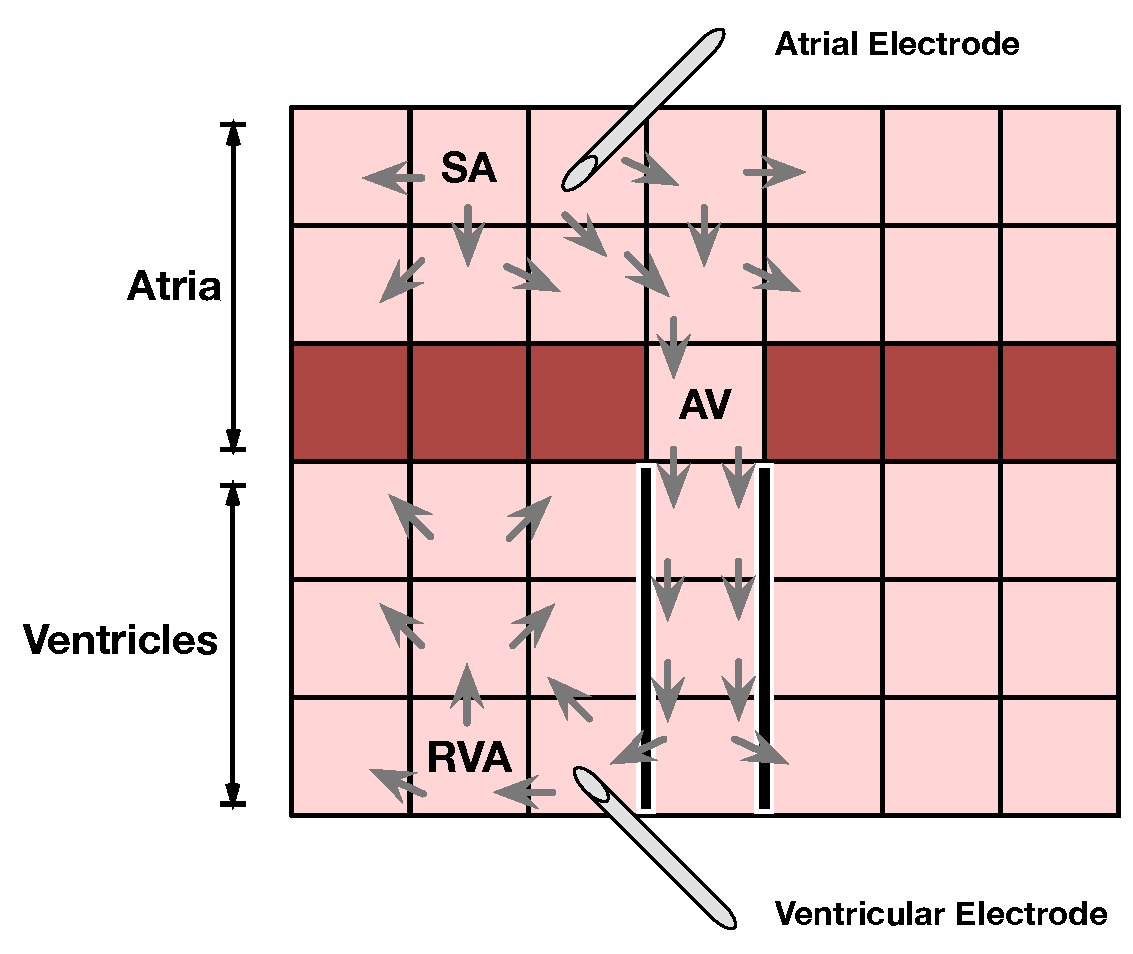
\includegraphics[scale=0.35]{figures/wholeHeartMesh}
%	\vspace{-10pt}
%	\caption{\small Whole heart modeled as a 2D mesh of cells. The \ac{ICD} leads are shown in the right atrium and ventricle. \textbf{AV}: atrio-ventricular node, \textbf{RVA}: right ventricle apex, \textbf{SA}: sino-atrial node.}
%	\label{fig:whole heart}
%	\vspace{-10pt}
%\end{figure}
The heart has two upper chambers called the \emph{atria} and two lower chambers called the \emph{ventricles} (Fig. \ref{fig:icd})
The synchronized contractions of the heart are driven by electrical activity.
Under normal conditions, the SinoAtrial (SA) node (a tissue in the right atrium) spontaneously \emph{depolarizes}, producing an electrical wave that propagates to the atria and then down to the ventricles (Fig.\ref{fig:overview})
In this model, the myocardium (heart's muscle) is treated as a 2D surface (so it has no depth), and discretized into \emph{cells}, which are simply regions of the myocardium (Fig. \ref{fig:overview}). 
Thus we end up with $N^2$ cells in a square $N$-by-$N$ grid.
A cell's voltage changes in reaction to current flow from neighboring cells, and in response to its own ion movements across the cell membrane.
This results in an \emph{\ac{AP}}.

Fig. \ref{fig:cellaut} shows how the \ac{AP} is generated by a given cell \cite{Klabunde_CVEPconcepts}:
in its quiescent mode (Phase 4), a cell $(i,j)$ in the grid has a cross-membrane voltage $V(i,j,t)$ equal to $V_{min} < 0$.
As it gathers charge, $V(i,j,t)$  increases until it exceeds a threshold voltage $V_th$.
The voltage then experiences a very fast increase, called the upstroke, to a level $V_{max} > 0$, after which it decreases to a plateau.
It stays at the plateau level for a certain amount of time \textbf{PD}  then decreases linearly to below $V_{th}$ (Phase 3 - ERP).
Once below $V_{th}$ it is said to be in the Relative Refractory Period (RRP).
In RRP, the cell can be depolarized a second time, albeit at a higher threshold $V_{th,2}$, slower and to a lower plateau level $V_{max,2} < V_{max}$.
Otherwise, when the voltage reaches $V_{min}$ again, the cell enters the quiescent stage again. 
This model is suitable for both pacemaker and non-pacemaker cells, the main differences being in the duration of the plateau (virtually non-existent for pacemaker cells), and the duration of phases 0 and 4 (both are shorter for pacemaker cells).

In Fig. \ref{fig:cellaut}, $V(i,j,t) \in \Re$ denotes the voltage in cell $(i,j)$ of the grid at time $t$, and vector $V =(V(1,1),\ldots, V(N^2,N^2))^T$ in $\Re^{N^2}$ groups the cross-membrane voltages of all cells in the heart.
The whole heart model $\Sys_{CA}$ is the parallel composition of these $N^2$ single-cell models. 
\begin{figure}[t]
	\centering
	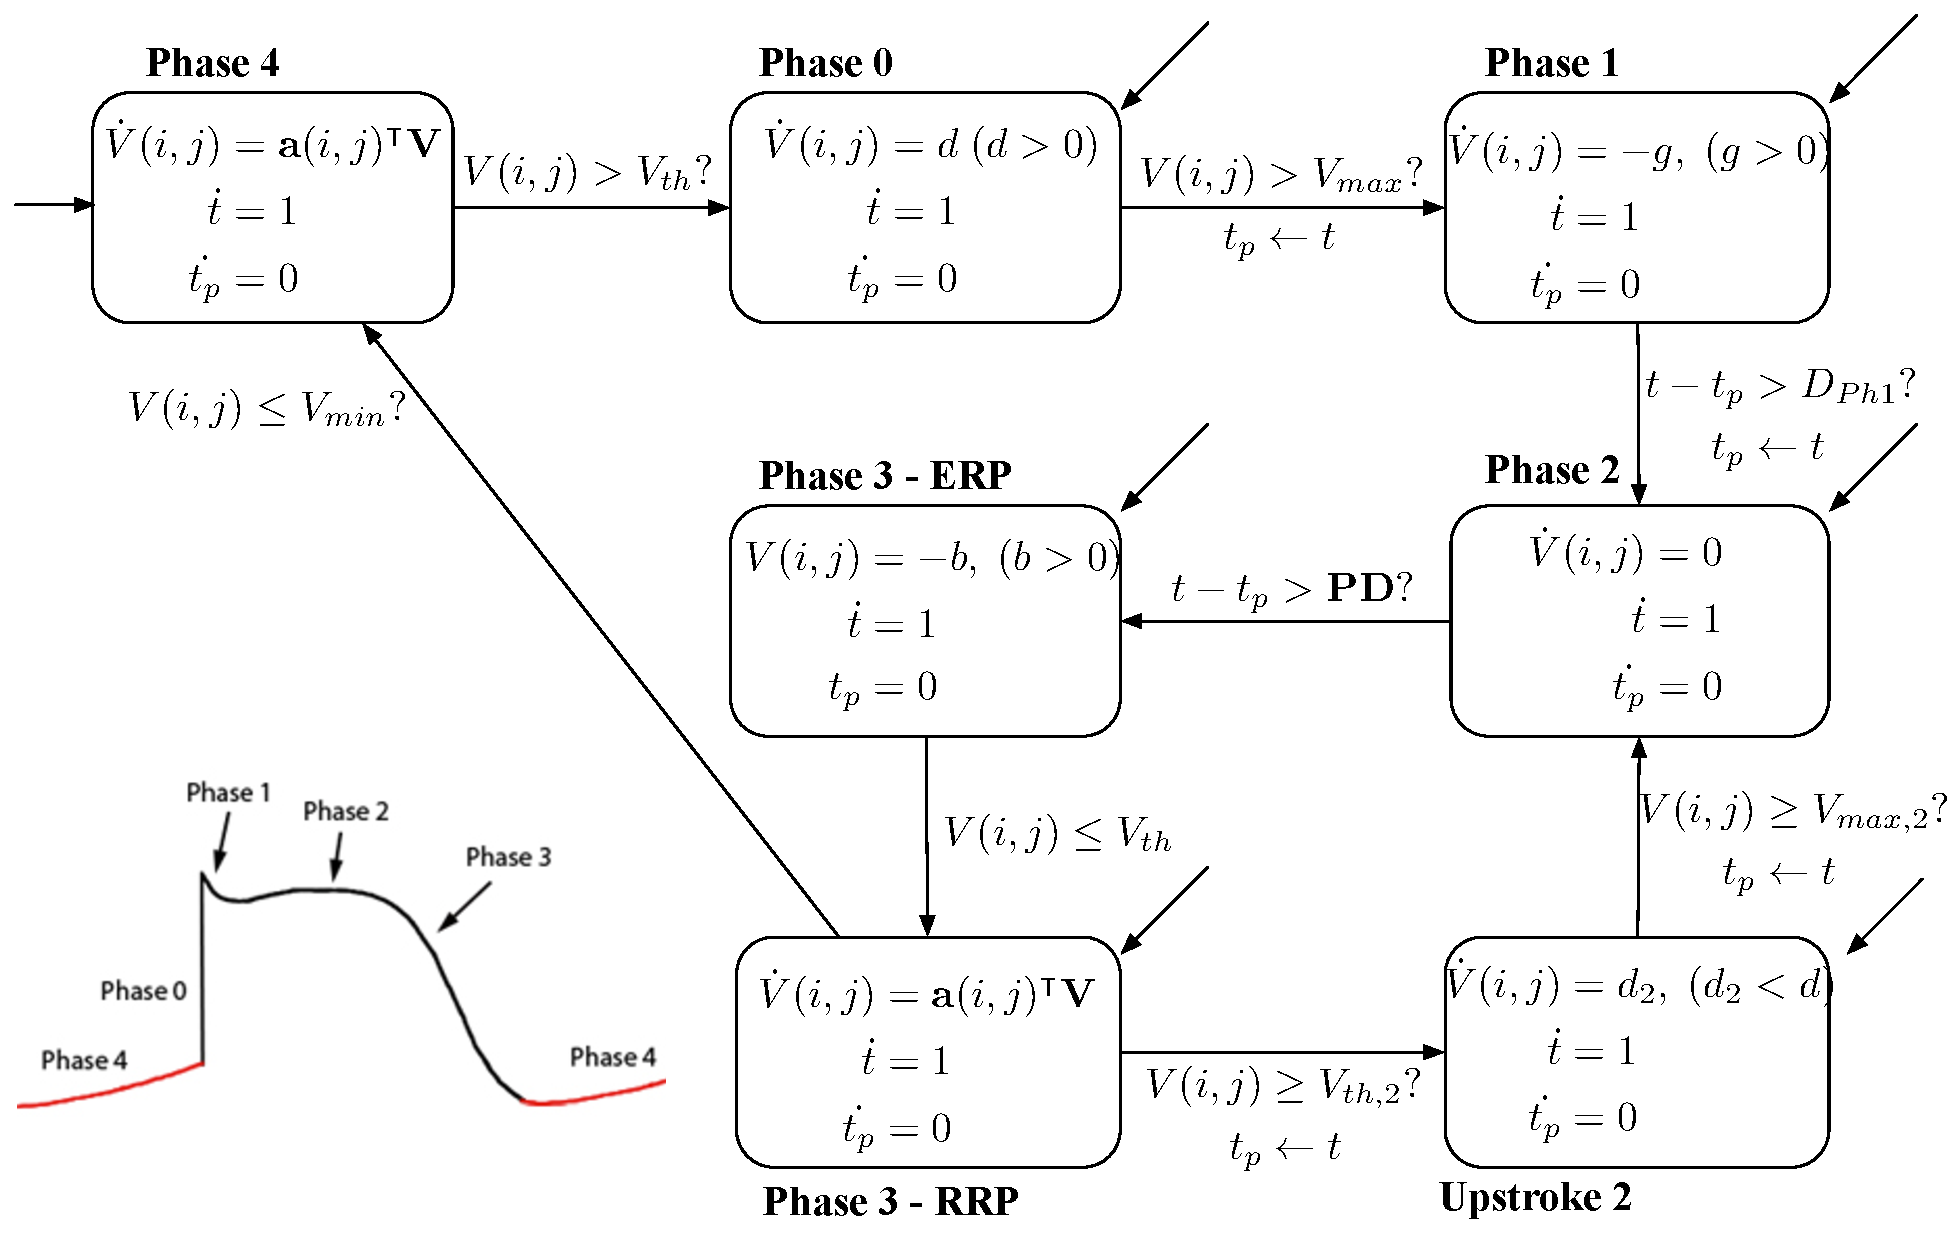
\includegraphics[scale=0.26]{figures/cellaut1v2}
	\vspace{-10pt}
	\caption{Hybrid model $\Sys_c$ of one cell of the heart model. AP figure from \cite{eplab}. 
		$V_{th,2}>V_{th}$, $V_{max,2}<V_{max}$}
	\vspace{-10pt}
	\label{fig:cellaut}
\end{figure}
%
The $(i,j)^{th}$ cell's voltage in Phase 4 depends on that of its neighbors and its own as follows \cite{Spector11_Emergence}
\begin{eqnarray}
\dot{V}(i,j,t) &=& \frac{1}{R_h}[V(i-1,j,t)+V(i+1,j,t) - 2V(i,j,t)] 
\nonumber \\ 
&& +  \frac{1}{R_v}[V(i,j-1,t) +  V(i,j+1,t) - 2V(i,j,t)]  
\nonumber\\
&=& a(i,j)^TV(t), \; a(i,j) \in \Re^{N^2}
\;
\end{eqnarray}
where $R_h$, $R_v$ are conduction constants that can vary across the myocardium.
Thus $V$ evolves according to a linear ODE $\dot{V} = AV$ where $A$ is the matrix whose rows are the $a(i,j)$. 
The two extra variables $t$ and $t_p$ are clocks.

\acp{ICD} observe the electrical activity through three channels (Fig.~\ref{fig:icd}).
Each signal is called an \ac{EGM} signal.
The signal read on a channel is the difference between two electrode potentials:
\begin{equation}
	\label{eq:vegm}
	\egm(t) = \frac{1}{K} \sum_{i,j} \left(\frac{1}{||(i,j)-p_0|| } - \frac{1}{||(i,j)-p_1||}\right) \dot{V}(i,j,t)
\end{equation}
where $p_0$ and $p_1$ are the electrodes positions.
This model was validated against real recordings taken in vitro \cite{StinnettDonnelly12_EGMresolution}.

\textbf{Extensions}. 
The APD restitution mechanism of heart cells, as modeled in \cite{Spector11_Emergence}, can be included in this model without changing its formal properties. 
%APD restitution models the dependence of the length of an \ac{AP} on the previous diastolic interval (roughly, the time between the end of one potential and the beginning of the next one).
%This is done in the online report.
%We used a simple constant slope for the variations of the \acp{AP}, as this was used in the original model \cite{Spector11_Emergence}. 
%Other more accurate shapes of the action potential are possible, while keeping the system STORMED.
%
%\subsection{Electrode measurement model}
%\label{sec:measurement}
%\acp{ICD} observes the electrical activity through three channels (Fig.~\ref{fig:icd}).
%Each signal is called an \ac{EGM} signal.
%The signal read on a channel is the difference between two potentials, and each potential may be modeled as being measured by an electrode located at position $p=(i_p,j_p)$ in the grid (Fig. \ref{fig:whole heart}).
%The potential measured by one electrode is given by \cite{StinnettDonnelly12_EGMresolution}:
%\begin{equation*}
%v_{E}(t) = \frac{1}{K} \sum_{i,j} \frac{I(i,j,t)}{||(i,j)-p||}
%\end{equation*}
%where $I(i,j,t)$ is the current density at $(i,j)$.
%In \cite{Spector11_Emergence} this current density is approximated as $I(i,j,t) \approx \dot{V}(i,j,t)$.
%%Thus we write 
%%\begin{equation}
%%\label{eq:apxI}
%%v_{E}(t) = \frac{1}{K} \sum_{i,j} \frac{\dot{V}(i,j,t)}{||(i,j)-p||}
%%\end{equation}
%We do not seek to verify the approximation - rather, we take it as our starting point.
%
%The \ac{EGM} signal is the difference of the two electrode potentials:
%\begin{equation}
%\label{eq:vegm}
%\egm(t) = \frac{1}{K} \sum_{i,j} \left(\frac{1}{||(i,j)-p_0|| } - \frac{1}{||(i,j)-p_1||}\right) \dot{V}(i,j,t)
%\end{equation}
%where $p_0$ and $p_1$ are the positions of the electrodes.
%This model was validated in vitro against real recordings taken by electrodes \cite{StinnettDonnelly12_EGMresolution}.

We now state and prove the main result of this section.
\begin{thm}
	Let $\Sys_{CA}$ be the whole heart cellular automaton model obtained by parallel composition of $N^2$ models $\Sys_c$ with state vector $x = [V, t,t_p,\egm ] \in \Re^{N^2}\times \Re^{3}$.
	Assume that all executions of the system have a duration of $D\geq 0$.
	Then $\Sys_{CA}$ is STORMED.
\end{thm}
\begin{prf}
	We verify each property of STORMED.
In this and all the proofs that follow, the approach is the same: $(ED)$ holds by Lemma \ref{prop:ED} because our state spaces are limited.
After establishing properties $(S), (T)$ and $(O)$, we draw up the constraints on $\phi$ and $\varepsilon$ imposed by reset and flow monotonicity (property (RM)). 
Then we argue that these constraints can be solved for $\phi$ and $\varepsilon$.
Often there is more than one solution and we just point to one.

\textbf{(S)} Separability holds because $V_{min} < V_{th}< V_{th,2} < V_{max,2} < V_{max}$ and $PD>0,D_{Ph_1}>0$. 
For example, on transition \textbf{Phase 4} $\rightarrow$ \textbf{Phase 0}, $V(i,j)=V_{th}$, which is separated from the next guard $\{V(i,j) > V_{max}\}$ by $|V_{max}-V_{th}|$.
%The only mode with two transitions is Phase 3 - RRP and its guards are $\{V(i,j) \leq V_{min}\}$ and $\{V(i,j) \geq V_{th,2}\}$ with separation $\sqrt{|V_{th,2}-V_{min}|}>0$.
\\
\textbf{(T)} All flows are linear or exponential and thus are TISG.
\\
\textbf{(O)} The flows, resets and guard sets are all definable in $\Lc_{\exp}$.
In particular the flow of $\dot{V} = AV$ is exponential with real exponent, and $\egm$ is a sum of exponentials and linear terms.
\\
\textbf{(RM)}
We seek a vector $\phi = (\phi_V,\phi_t,\phi_p,\phi_\egm)^T \in \Re^{N^2+3}$ such that resets and flows are monotonic along $\phi$.
Only transitions $p \rightarrow q \neq p$ are to be found in $\Sys_{CA}$, during which only $t_p$ is reset. 
Always, $t_p^+ = t \geq t_p^-$, thus the reset is indeed monotonic as can be seen by choosing any $\varepsilon >0$ and $\phi_p > \varepsilon$.

Monotonic flows: $\phi$ must also be such that in all modes:
\begin{equation*}
\phi \cdot (\theta_\ell(t+\tau;x) - \theta_\ell(t;x)) \geq \varepsilon ||\theta_\ell(t+\tau;x) - \theta_\ell(t;x)||
\end{equation*}
Decomposing, we want 
\begin{eqnarray*}
\label{eq:monotonic flow ca}
&&\phi_V \cdot(V(t+\tau) - V(t)) + \phi_t \tau + \phi_p \cdot 0 \\
&&\quad+ \phi_\egm \cdot (\egm(x,t+\tau) - \egm(x,t)) \geq \varepsilon ||\theta_\ell(x,t+\tau) - \theta_\ell(x,t)||
\end{eqnarray*}
Now note that all flows have bounded derivatives in every bounded duration of flow and are thus Lipschitz. 
Let $L_V$ be the Lipshitz constant of $V(t)$ and $L_{\egm}$ that of $\egm(t)$.
Then on the LHS of the above inequality we have 
$\phi_V \cdot(V(t+\tau) - V(t)) + \phi_\egm \cdot(\egm(t+\tau) - \egm(t)) \geq -\phi_V L_V \tau  -\phi_\egm L_{\egm} \tau$.
On the RHS we have  
$\varepsilon (L_V\tau + L_{\egm}\tau + \tau) \geq \varepsilon ( ||V(t+\tau) - V(t)|| + ||\egm(t+\tau) - \egm(t) ||  + \tau) \geq \varepsilon ( ||\theta_\ell(x,t+\tau) - \theta_\ell(x,t)||)$
Thus \eqref{eq:monotonic flow ca} is satisfied if the stronger inequality 
\[-\phi_V L_V \tau  -\phi_\egm L_{\egm} \tau + \phi_t \tau \geq \varepsilon (L_V\tau + L_{\egm}\tau + \tau) \]
is satisfied.
But this can be achieved by, for example, choosing $\phi_V = \phi_\egm = 0$ and $\phi_t \geq \varepsilon(L_V+L_{\egm}+1)$.
\\
\textbf{(ED)} Our system has bounded state spaces: $V$ and $\egm$ are voltages typically in the range $[-80,60]$ mV and $t_p \leq t \leq D$.
So (ED) holds by Lemma \ref{prop:ED}. 
\end{prf}
\section{ICD Sensing}
\label{sec:sensing}
\begin{figure}[t]
	\centering
	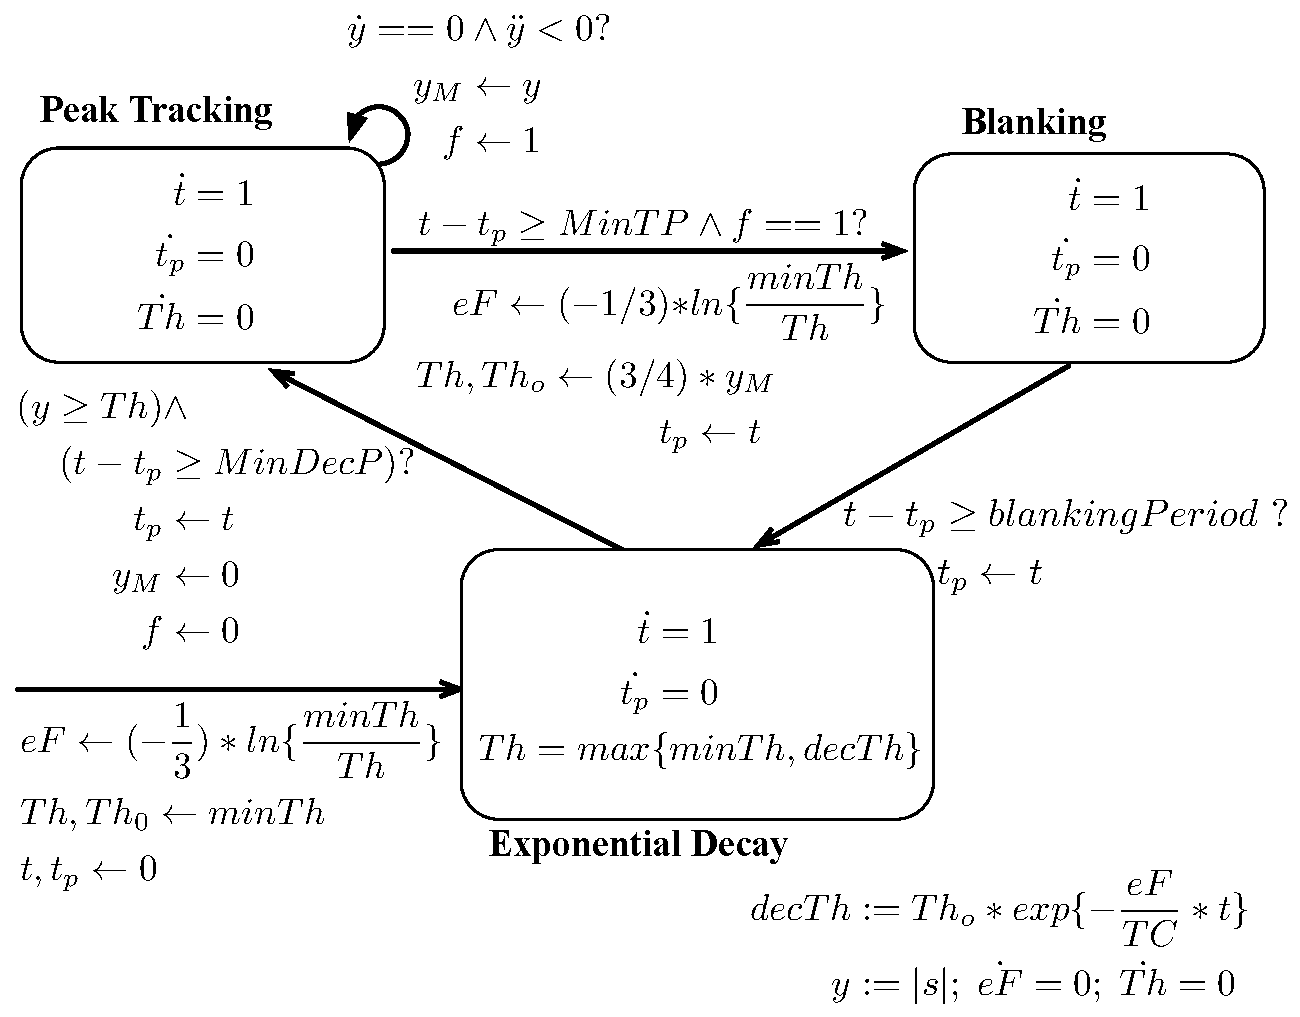
\includegraphics[scale=0.35]{figures/sensingModel}
	\vspace{-10pt}
	\caption{\small $\Sys_{Sense}$. States not shown in a mode have a 0 derivative, e.g., $\dot{eF}=0$ in all modes.}
	\vspace{-10pt}
	\label{fig:sensingModel}
\end{figure}
\begin{figure}[t]
	\centering
	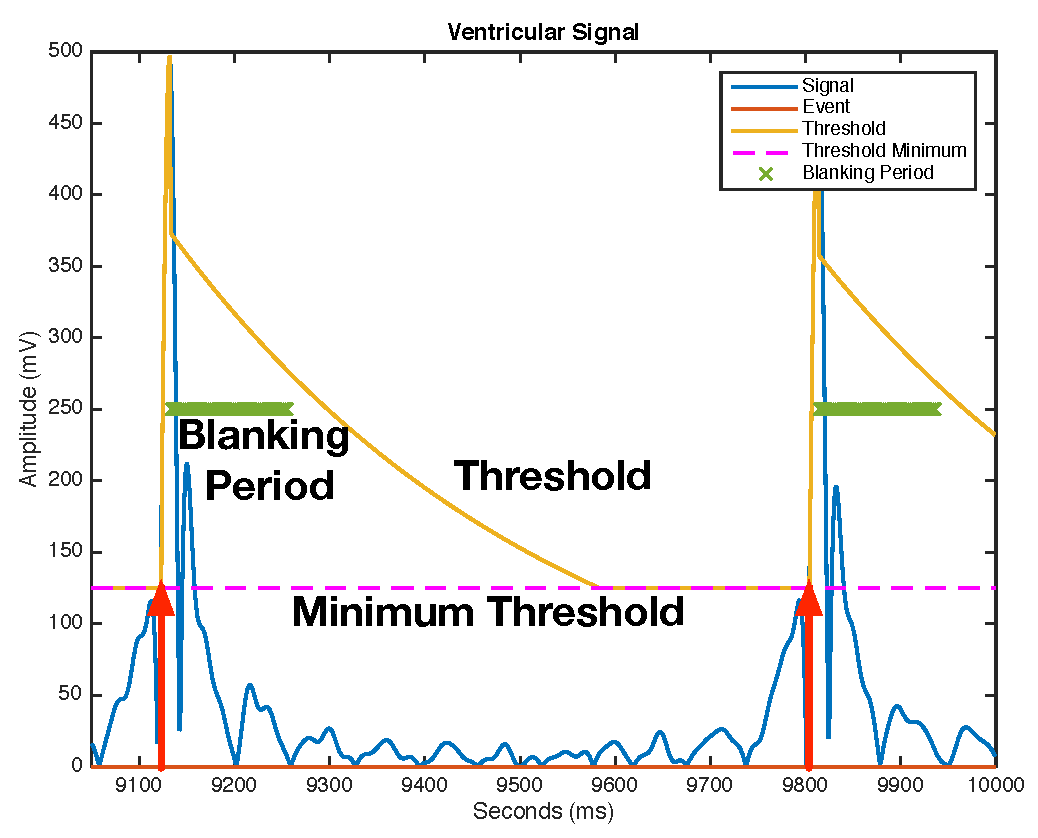
\includegraphics[scale=0.3]{figures/sensingExample}
	\vspace{-10pt}
	\caption{\small Example of dynamic threshold adjustment in ICD sensing algorithm. The shown signal is rectified.}
	\vspace{-10pt}
	\label{fig:sensingExample}
\end{figure}

\emph{Sensing} is the process by which cardiac signals $\egm$ measured through the leads of the \ac{ICD} are converted to cardiac timing events.
The \ac{ICD} sensing algorithm is a threshold-based algorithm which declares events when the signal exceeds a dynamically-adjusted threshold $Th$.
%The threshold is dynamically adjusted in order to operate robustly in complex environments where cardiac events can vary greatly in signal amplitude and frequency, such as during \ac{VF}.

Fig. \ref{fig:sensingModel} shows the model $\Sys_{Sense}$ of the sensing algorithm, and Fig. \ref{fig:sensingExample} illustrates its operation. 
%In Fig. \ref{fig:overview} (ICD Sensing - $\Sys_{Sense}$), states not shown in a mode have a 0 derivative, e.g., $\dot{eF}=0$ in all modes. $y(t) = |\egm(t)|$.
The sensing takes place on the rectified \ac{EGM} signal $y = |\egm|$.
After an event is declared at the current threshold value ($y(t)\geq Th(t)$ in Fig. \ref{fig:sensingModel}), the algorithm tracks the signal in order to measure the next peak's amplitude \yhl{(Peak Tracking)}.
%During transition, the state to indicate peak discovery is reset ($f=0$). 
For a duration $MinTP$ (min tracking period) the latest peak is saved in $y_M$.
A variable $f$ indicates that a peak was found.
After a peak is found ($f==1$) and after the end of the tracking period, the algorithm enters a fixed \emph{Blanking Period} \yhl{(Blanking)}, during which additional events are ignored.
\yhl{On the transition to Blanking}, $Th$ and $Th_0$ are set to 3/4 the current value of $y_{M}$ and the exponential factor of decay is updated ($eF=(-1/3)*ln{\frac{minTh}{TH}}$). 
At the end of the blanking period, the algorithm then transitions to the Exponential Decay mode in which $Th$ decays exponentially from $Th_0$ to a minimum level \yhl{(Exponential Decay)}:
$Th(t) = \max(minTh, Th_0\cdot exp(-(eF/TC)t)) $.
The algorithm stays in the Exponential Decay mode for at least a sampling period of $MinDecP$.
Correspondingly, there is a de facto Maximum Decay Period $MaxDecP$ after which the system transitions again to PeakTracking since the signal $y$ is bound to exceed the minimum threshold $minTh$.
Different manufacturers may use a step-wise decay instead of exponential, but the principle is the same.
%
Local peak detection is modeled via the $\dot{y} = 0 \wedge \ddot{y}<0$ transition.
While $y=|\egm|$ is non-differentiable at 0, the peak will occur away from 0, as shown in Fig. \ref{fig:sensingExample}.
The other states in Fig. \ref{fig:sensingModel} are $t, t_p$ (clocks).
$minTh$ and $TC$ are constant parameters.
\begin{thm}
	\label{thm:sensing}
	$\Sys_{Sense}$ is STORMED.	
\end{thm}
\begin{prf}
	\textbf{(S)} By definition, we only need to consider transitions between different modes to establish separability. 
	For all such transitions, there is a minimum dwell time in the mode before taking the transition, namely $MinTP$ in PeakTracking, $BlankingPeriod$ in Blanking, and  $MinDecP$ in mode ExponentialDecay.
	So the system is separable since there is a uniform minimum flow before jumping.
	\\
	\textbf{(T)} Flows are either constant, (piece-wise) linear, or piece-wise linear and exponential (in the case of $y$ and its derivatives) and therefore are TISG.
	\\
	\textbf{(O)} All the flows, resets and guard sets are definable in $\Lc_{\exp}$.
	(The absolute value and $\max$ functions can be broken down into boolean disjunctions of definable functions, and $t \mapsto \ln(t)$ is o-minimal by o-minimality of $\exp$).
	\\
	\textbf{(RM)} The state is $x = (t, t_p, y, y_M, f, Th, Th_0,eF) \in \Re^8$, and let 
	 $\phi = (\phi_t, \phi_{p}, \phi_y, \phi_m, \phi_f, \phi_{Th},\phi_0,\phi_{eF})$ be the corresponding $\phi$ vector.
	Recall that the \ac{EGM} voltage $\egm$, and so $y=|s|$, is upper-bounded by $V_M$.	
	\\ 
	\textbf{ExponentialDecay $\rightarrow$ PeakTracking}.
	Only $t_p,y_M$ and $f$ are modified, so monotonicity produces the constraint
	 $\phi_p(t-t_p) +\phi_m(0-y_M) + \phi_f(0-1) \stackrel{Want}{\geq} \varepsilon (|t-t_p|+|y_M|+1)$.
	We require the stronger constraint to hold:
	\[\phi_t MinDecP - \phi_m V_M -\phi_f \stackrel{Want}{\geq} \varepsilon(MaxDecP + V_M+1)\]
	\\
	\textbf{PeakTracking $\rightarrow$ PeakTracking}. Only $y_M$ and $f$ are reset. 
	Algebraic manipulation yields $-2V_M\phi_m + \phi_f \stackrel{Want}{\geq} \zeta$
	\\
	\textbf{PeakTracking $\rightarrow$ Blanking}.
	$t_p,eF,Th$ and $Th_0$ are reset, so we get
	\begin{eqnarray*}
	&&\;\phi_p(t-t_p) + \phi_{eF}(-(1/3)\ln(minTh/Th)-eF) 
	\\
	&&+\phi_{Th}(3y_M/4-Th) +\phi_0(3y_M/4-Th_0)
	\\
	&&\geq \varepsilon(|t-t_p|+ |-\frac{1}{3}\ln(\frac{minTh}{Th})-eF|
	\\
	&&+|\frac{3y_M}{4}-Th|+|\frac{3y_M}{4}-Th_0|)
	\end{eqnarray*}
	
	$Th$ is lower-bounded by $minTh$ at all times, and it is naturally upper-bounded by $V_M$ as the threshold should never exceed the largest possible attainable voltage. 
	By the same token, $0\leq eF \leq (1/3)\ln(V_M/minTh)$.
	Then we want the stronger inequality
	\begin{eqnarray*}
	\phi_p MinTP &+& \phi_{eF}(0-(1/3)\ln(V_M/minTh)
	\\
	&+&\phi_{Th}(-V_M) +\phi_0(-V_M)
	\\
	&\geq& \varepsilon(MaxTP+ |\frac{1}{3}\ln(\frac{V_M}{Th})|+|V_M|+|V_M|)
	\end{eqnarray*}
	\\
	\textbf{Blanking $\rightarrow$ ExponentialDecay}. Only $t_p$ is reset and therefore we want, $\phi_p(t-t_p) \geq \varepsilon(|t-t_p|)$, thus the transition yields $\phi_p \geq \varepsilon$.
	
	The above equations can be simultaneously satisfied.
	The simplest thing would be to set all $\phi$ terms that appear above to 0 except for $\phi_t,\phi_p$ which are calculated accordingly.
	
	The flows can be shown to be monotonic along the same $\phi$ and with the same $\varepsilon$.
	For example, in mode ExponentialDecay, only $t,y$ and $Th$ flow.
	Making use of the $V_M$ bound on $y$, we get the constraint
	$\phi_t \tau - 2V_M\phi_y +\phi_{Th}(Th(t+\tau)-Th(t))\geq \varepsilon(\tau+2V_M + |Th(t+\tau)-Th(t)| )$, 
	which yields $\phi_t \geq \varepsilon$, $\phi_y \leq -\varepsilon$ and $\phi_{Th} \geq \varepsilon$. 
	Similarly for the rest.	
\end{prf}

%\begin{thm}
%\label{thm:sensing}
%$\Sys_{Sense}$ is STORMED.	
%\end{thm}
%\begin{prf}
%\textbf{(S)} The guards are separable since each mode has only one guard.
%\\
%\textbf{(T)} The flows are constant, linear or equal to $\pm \egm(t)$ (in the case of $y$) and so are TISG.
%\\
%\textbf{(O)} All the flows, resets and guard sets are definable in $\Lc_{\exp}$.
%(The absolute value and $\max$ functions can be broken down into boolean disjunctions of definable functions).
%In particular, $t \mapsto \ln(t)$ is o-minimal by o-minimality of $\exp$.
%\\
%\textbf{(RM)} The only reset happens on the PeakTracking $\rightarrow$ Blanking transition. 
%The state is $x = (t,Th, eF,Th_0,t_p,y) \in \Re^5$.
%We seek a vector $\phi = (\phi_t, \phi_{Th}, \phi_{eF},\phi_0,\phi_y)$ and $\varepsilon >0$ s.t. 
%\begin{equation}
%\label{eq:sense rm}
%\phi \cdot \left(\begin{matrix}
%t-t \\ (3/4)Th-Th\\ -(1/3)\ln(minTh/Th) - eF\\ (3/4)Th-Th_0\\ t-t_p \\ y-y
%\end{matrix}
%\right) \defeq \phi \cdot \delta \stackrel{Want}{\geq} \varepsilon ||\delta||
%\end{equation} 
%$Th$ is lower-bounded by $minTh$ at all times, and it naturally has an upper bound, since it doesn't make sense to set it above the largest possible voltage. 
%Let that maximum be $maxTh$.
%Then we want the stronger inequality
%\begin{eqnarray*}
%&&\phi_{Th}(-Th/4) + \phi_{eF}(-(1/3)ln(minTh/Th)-eF) 
%\\
%&+& \phi_0(3Th/4-Th_0) + \phi_t (t-t_p) \geq ||\delta||
%\\
%&\geq& -\frac{\phi_{Th}}{4}maxTh + \phi_{eF}(-\frac{2}{3}\ln(minTh/Th)) 
%\\
%&& -\phi_0(2maxTh) + \phi_p(t-t_p)
%\\
%&\stackrel{Want}{\geq}& \varepsilon \left(|\frac{maxTh}{4}| + |\frac{2}{3}\ln(\frac{minTh}{Th})| + |2maxTh| +  \phi_p|t-t_p|\right)
%\end{eqnarray*}
%Since the $\ln$ term is negative and $t\geq t_p$,this yields the constraints:
%$\phi_0,\phi_{Th} < -\varepsilon \text{  and  } \phi_{eF},\phi_t > \varepsilon$.
%%\begin{equation}
%%\label{eq:constraint sense rm}
%%\phi_0,\phi_{Th} < -\varepsilon \text{  and  } \phi_{eF},\phi_t > \varepsilon
%%\end{equation}
%
%The flows are also monotonic along the same $\phi$ and with the same $\varepsilon$.
%For any $t,\tau>0$ and $x\in \stSet$, flow monotonicity is implied by the stronger inequality
%\begin{equation}
%\label{eq:sense fm}
%\phi \cdot \left(\begin{matrix}
%t+\tau-t \\ Th-Th\\ eF - eF\\ Th_0-Th_0\\ t_p-t_p \\ |\egm(t+\tau)|-|\egm(t)|
%\end{matrix}
%\right) \stackrel{Want}{\geq} \varepsilon (\tau + \underbrace{||\egm(t+\tau)|-|\egm(t)||}_{\delta \egm})
%\end{equation} 
%$\implies \phi_t \tau + \phi_y (|\egm(t+\tau)|-|\egm(t)|) \geq \varepsilon (\tau + \left| |\egm(t+\tau)|-|\egm(t)| \right| )$
%Therefore we can choose $\phi_t > \varepsilon$ as before and $\phi_y < -\varepsilon$.
%%We show this for Mode 1 only, the other modes are dealt with similarly.
%%\underline{Mode 1.} For any $t,\tau>0$ and $x\in \stSet$, flow monotonicity 
%%$\phi\cdot(\theta(t+\tau;x)-\theta(t;x)) \geq \varepsilon ||\theta(t+\tau;x)-\theta(t;x)||$ is implied by the stronger inequality
%%\begin{equation}
%%\label{eq:sense fm}
%%\phi \cdot \left(\begin{matrix}
%%t+\tau-t \\ Th-Th\\ eF - eF\\ Th_0-Th_0\\ t_p-t_p \\ -\egm(t+\tau)+\egm(t)
%%\end{matrix}
%%\right) \stackrel{Want}{\geq} \varepsilon (\tau + \underbrace{|\egm(t)-\egm(t+\tau)|}_{\delta \egm})
%%\end{equation} 
%%Observing that the \ac{EGM} signal $\egm$ has naturally defined minimum $\egm_{min}$ and maximum $\egm_{max}$, \eqref{eq:sense fm} is further implied by 
%%\begin{equation}
%%\phi_t\tau + \phi_y(\delta \egm) \geq \phi_t \tau - \phi_y(s_{min} -  s_{max}) \stackrel{Want}{\geq} \varepsilon (\tau +|s_{min} -  s_{max}|)
%%\end{equation}
%%which yields the constraints $\phi_t > \varepsilon, \phi_y < -\varepsilon$, which are consistent with \eqref{eq:constraint sense rm}.
%%The flow monotonicity constraints from the other modes are similarly consistent with \eqref{eq:constraint sense rm}. 
%\end{prf}

\section{Arrhythmia detection}
\label{sec:discriminators}
Because a sustained \ac{VT} (or \ac{VF}) can be fatal whereas an \ac{SVT} is usually not fatal, 
\emph{the ICD's main task is to discriminate \ac{VT} from \ac{SVT} and deliver therapy to the former only} \cite{compass}.
%\emph{\ac{VT}} is an example of a tachycardia originating in the ventricles, in which the ventricles spontaneously beat at a very high rate.
%If the \ac{VT} is sustained, or degenerates into \ac{VF}, it can be fatal.
%A tachycardia that originates above the ventricles is referred to as a \emph{\ac{SVT}} and is a diseased but non-fatal condition.
%In what follows, we will refer to sustained \ac{VT} and \ac{VF} together as \ac{VT}.
%\emph{The ICD's main task is to discriminate \ac{VT} from \ac{SVT} and deliver therapy to the former only}.
Most \ac{VT}/\ac{SVT} detection algorithms found in ICDs today are composed of individual \emph{discriminators}. 
A discriminator is a software function whose task is to decide whether the current arrhythmia is \ac{SVT} or \ac{VT}.
No one discriminator can fully distinguish between SVT and VT.
Thus a detection algorithm is often a decision tree built using a number of discriminators \emph{running in parallel}.
We have modeled each discriminator in this detection algorithm as a STORMED hybrid system.
The algorithm itself is then a hybrid system.
\textbf{The ICD system is thus 
$\mathbf{\Sys_{ICD} = \Sys_{Sense}||\Sys_{Detection-Algo}}$ where $\mathbf{\Sys_{Detection-Algo}}$ is the parallel composition of the discriminator systems}.
In what follows, we present two of these discriminators we modeled, which are found in most ICDs and model them as hybrid systems, and prove they are STORMED.

\subsection{Three Consecutive Fast Intervals}
\label{sec:tcfi}
\begin{figure}[t]
	\centering
	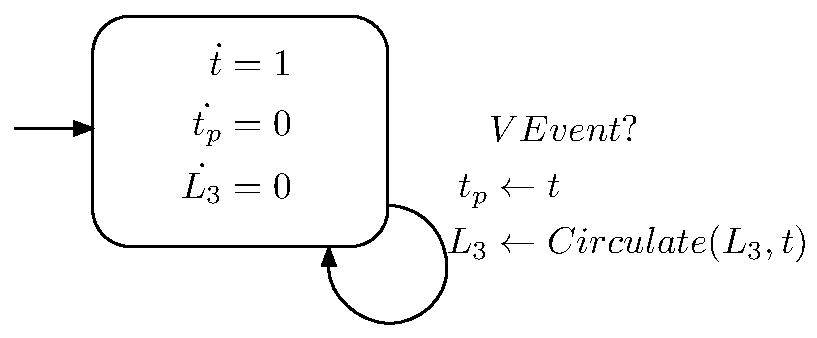
\includegraphics[scale=0.3]{figures/TCFI}
		\vspace{-10pt}
	\caption{Three Consecutive Fast Intervals $\Sys_{TCFI}$}
	\label{fig:tcfi}
\end{figure}
Our first module simply detects whether three consecutive fast intervals have occurred, where `fast' means the interval length, measured between 2 consecutive peaks on the \ac{EGM} signal, is shorter than some pre-set amount.
See Fig. \ref{fig:tcfi}.
States $t$ and $t_p$ are clocks as before.
The vector $L_3$ is three-dimensional, and stores the values of the last three intervals.
The event VEvent? is shorthand for the transition $y(t) \geq Th$ being taken by the $\Sys_{Sense}$ automaton.
In other words, it indicates a ventricular event.
Then $L_3$ gets reset to $L_3^+ = (z_1,z_2,z_3)^+ \defeq \text{Circulate}(L_3,t-t_p)$ where
\begin{equation}
L_3^+ = 
\left(\begin{matrix}
z_2\\z_3\\t-t_{p}\\
\end{matrix}
\right)
=
\left(\begin{matrix}
0 & 1 & 0\\0& 0& 1\\0& 0 &0
\end{matrix}
\right) L_3 + 
\left(\begin{matrix}
0\\0\\t-t_p
\end{matrix}
\right)
\end{equation}
%
\begin{lemma}
	$\Sys_{TCFI}$ is STORMED.
\end{lemma}


\subsection{Vector Timing Correlation}
\label{sec:VTC}
\begin{figure}[t]
	\centering
	\vspace{-15pt}
	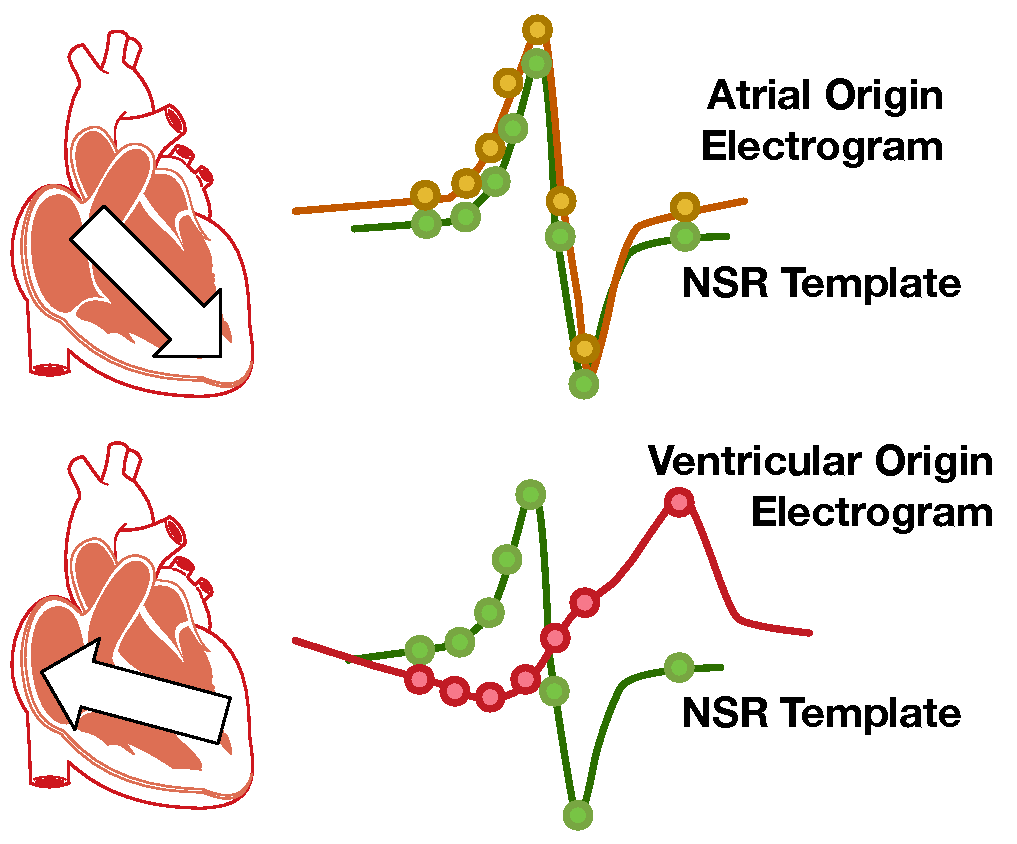
\includegraphics[scale=0.3]{figures/VTCEGMCompare}
	\caption{\small \acp{EGM} of different origin have different morphologies.}
	\label{fig:egmmorphology}
	\vspace{-10pt}
\end{figure}
%\caption{\small \acp{EGM} of different origin have different morphologies, while \acp{EGM} of same origin have very similar morphologies.}
It has been clinically observed that a depolarization wave originating in the ventricles (as produced during \ac{VT} for example) will in general produce a different \ac{EGM} morphology than a wave originating in the atria (as produced during \ac{SVT}) \cite{compass}.
See Fig. \ref{fig:egmmorphology}.
%
A morphology discriminator measures the correlation between the morphology of the current \ac{EGM} and that of a stored \emph{template} \ac{EGM} acquired during normal sinus rhythm.
If the correlation is above a pre-set threshold for a minimum number of beats, then this is an indication that the current arrhythmia is supraventricular in origin.
Otherwise, it might be of ventricular origin.

Boston Scientific's implementation of a morphology discriminator is called Vector and Timing Correlation (VTC).
VTC first samples 8 \emph{fiducial} points $\egm_i,i=1,\ldots,8$ on the current \ac{EGM} $\egm$ at pre-defined time instants.
Let $\egm_{m,i}$ be the corresponding points on the template \ac{EGM}.
A simple 0-shift correlation $\rho_{new}$ is calculated between the two sequences. 
If 3 out of the last 10 calculated correlation values exceed the threshold, then \ac{SVT} is decided and therapy is withheld.

The system of Fig. \ref{fig:HVTC} implements the VTC discriminator.
As before, $t$ is a local clock.
$\mu$ accumulates the values of the current \ac{EGM}, $\alpha$ accumulates the product $\egm_i \egm_{m,i}$, 
$\beta$ accumulates $\egm_i^2$.
State $w$ is an auxiliary state we need to establish the STORMED property.
$\vec{\nu}$ is a 10D binary vector: $\nu_i = -1$ if the $i^{th}$ correlation value fell below the threshold, and is $+1$ otherwise.
$L_3$ is the state of $\Sys_{TCFI}$: the guard condition $L_3 \leq th$ indicates that all its entries have values less than the tachycardia threshold, which is when $\Sys_{VTC}$ starts computing.
$WindowEnds$ indicates the `end' of an \ac{EGM}, measured as a window around the peak sensed by $\Sys_{Sense}$.  
%
\begin{figure}[t]
\centering
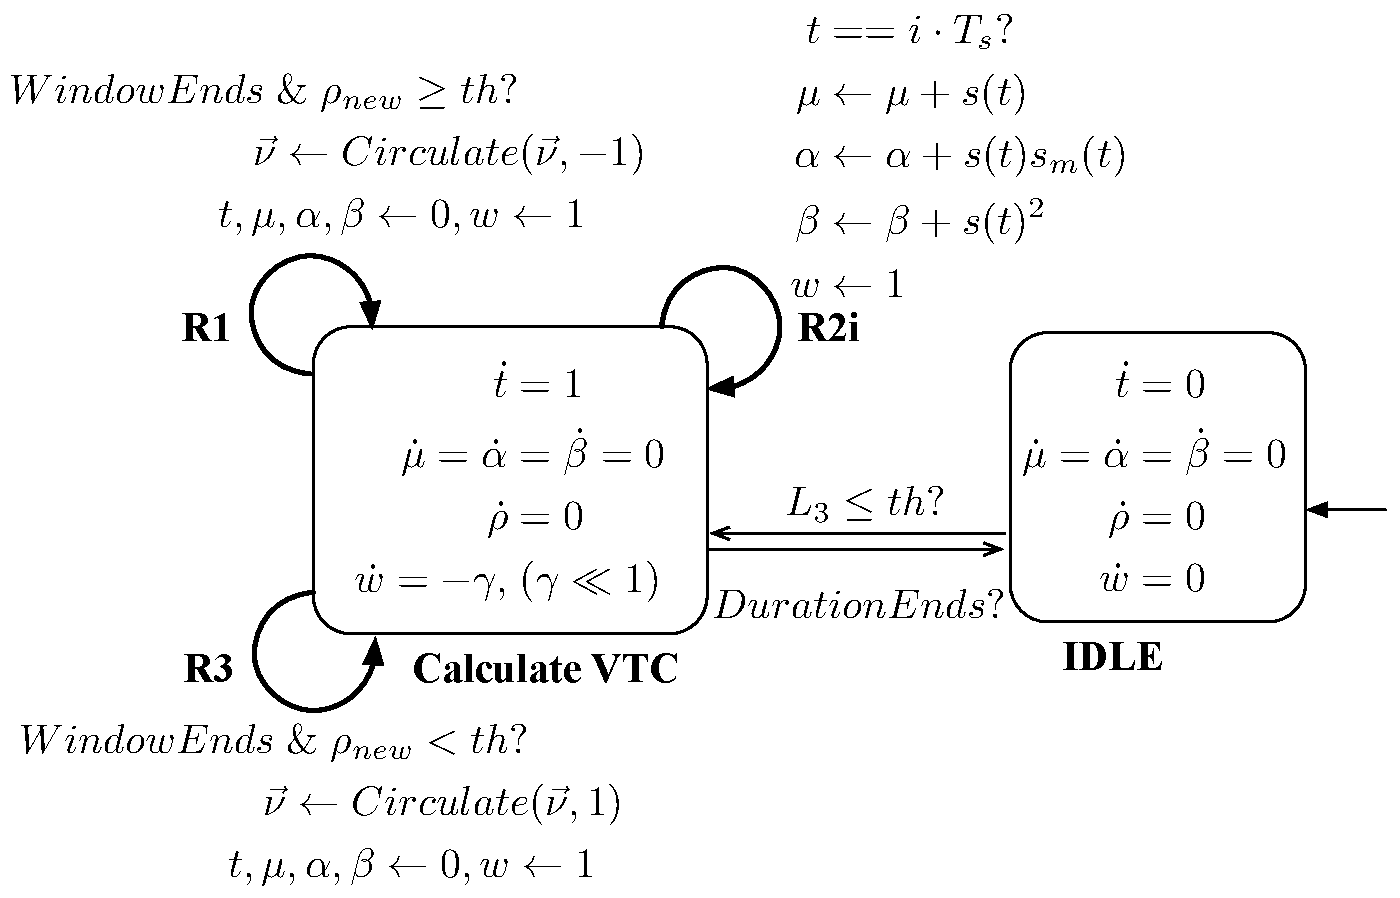
\includegraphics[scale=0.325]{figures/VTC1v2}
\vspace{-10pt}
\caption{VTC calculation. $iT_s$ is the sampling time for the $i${th} fiducial point, $i=1,\ldots,8$. $R2_{1},\ldots,R2_{8}$ are the corresponding resets. For clarity of the figure, 8 transitions are represented on the same edge.}
\vspace{-10pt}
\label{fig:HVTC}
\end{figure}
%
\begin{lemma}
	\label{lemma:vtc}
	$\Sys_{VTC}$ is STORMED.
	\end{lemma}

\subsection{Stability discrimination}
\label{sec:stability}
%\begin{figure}[t]
%	\centering
%	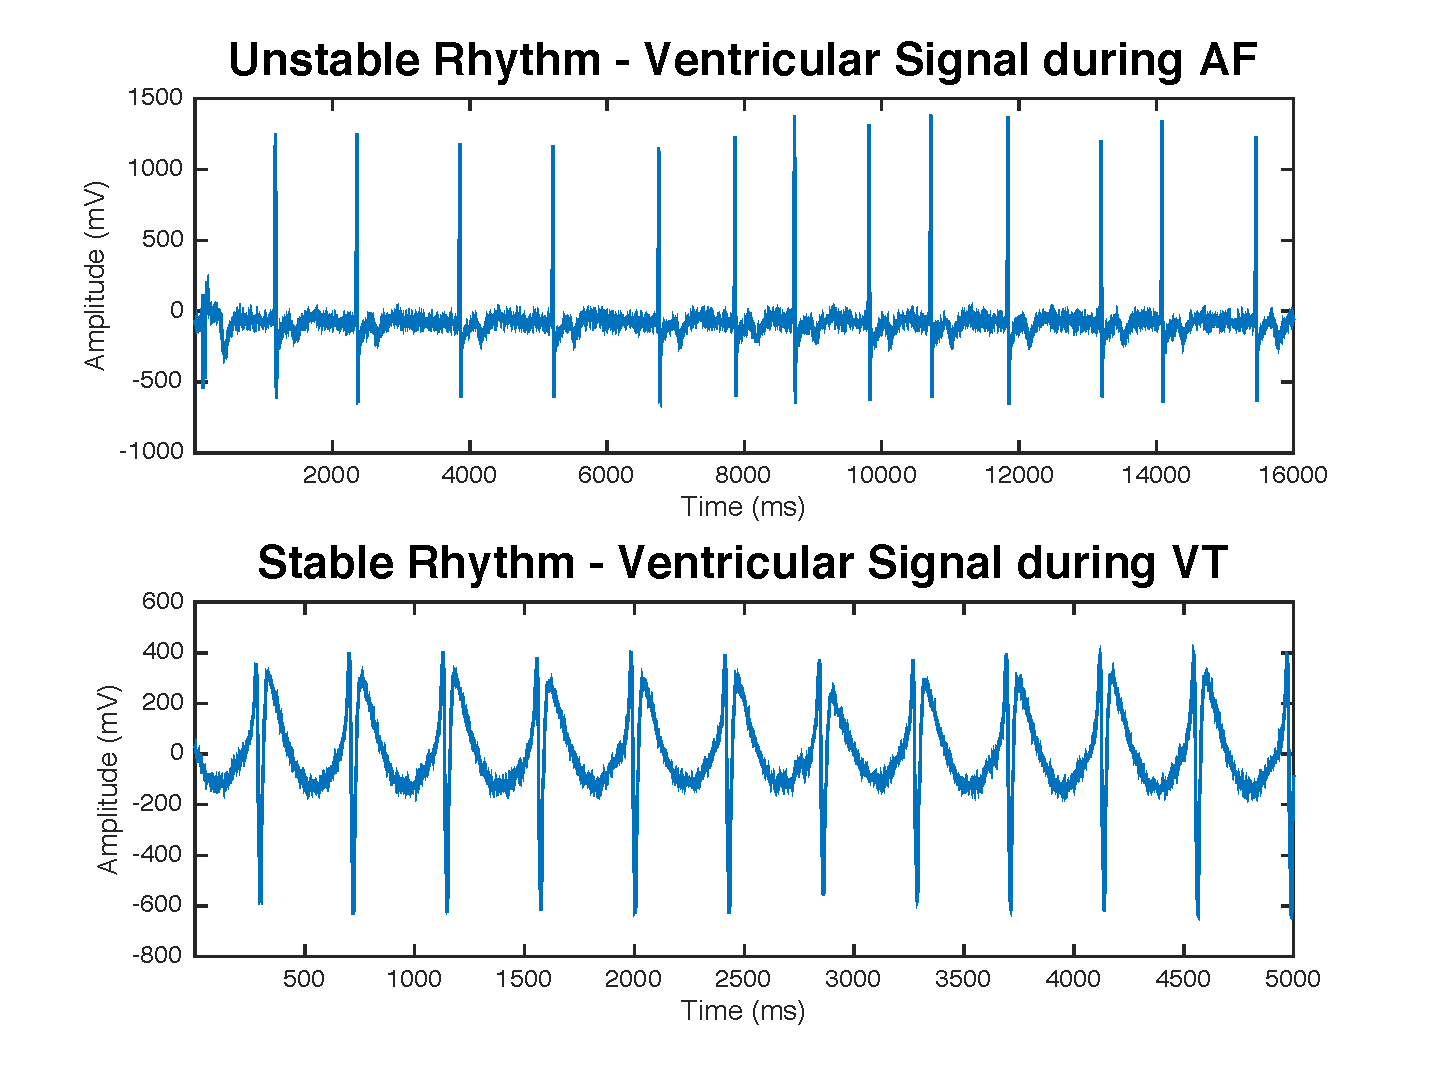
\includegraphics[scale=0.35]{figures/EGMStability}
%	\caption{Examples of a unstable rhythm (top) and stable rhythm (bottom).}
%	\label{fig:stable unstable}
%\end{figure}
\emph{Stability} refers to the variability of the peak-to-peak cycle length.
A rhythm with large variability (above a pre-defined threshold) is said to be \emph{unstable}, and is called stable otherwise.
The Stability discriminator is used to distinguish between atrial fibrillation, which is usually unstable, and \ac{VT}, which is usually stable.
%Atrial fibrillation, which is usually unstable, might induce a high ventricular rate .
%A \ac{VT}, on the other hand, is usually stable.
%Therefore this is a useful discriminator.

The Stability discriminator shown in Fig. \ref{fig:Hstab} simply calculates the variance of the cycle length over a fixed period called a Duration (measured in seconds).
Let $DL \geq 0$ be the Duration length.
The event $DurationEnds?$ indicates a transition of a simple system that measures the lapse of one Duration (not shown here).
State $t$ is a clock, $L_1$ accumulates the sum of interval lengths (and will be used to compute the average length), 
$L_2$ accumulates the squares of interval lengths,
and $\kappa$ is a counter that counts the number of accumulated beats.
$\sigma_2$ is assigned the value of the variance given by $\frac{1}{\kappa}[L_2 - 2L_1/\kappa + \kappa(L_1/\kappa)^2]$
\begin{figure}[t]
	\centering
	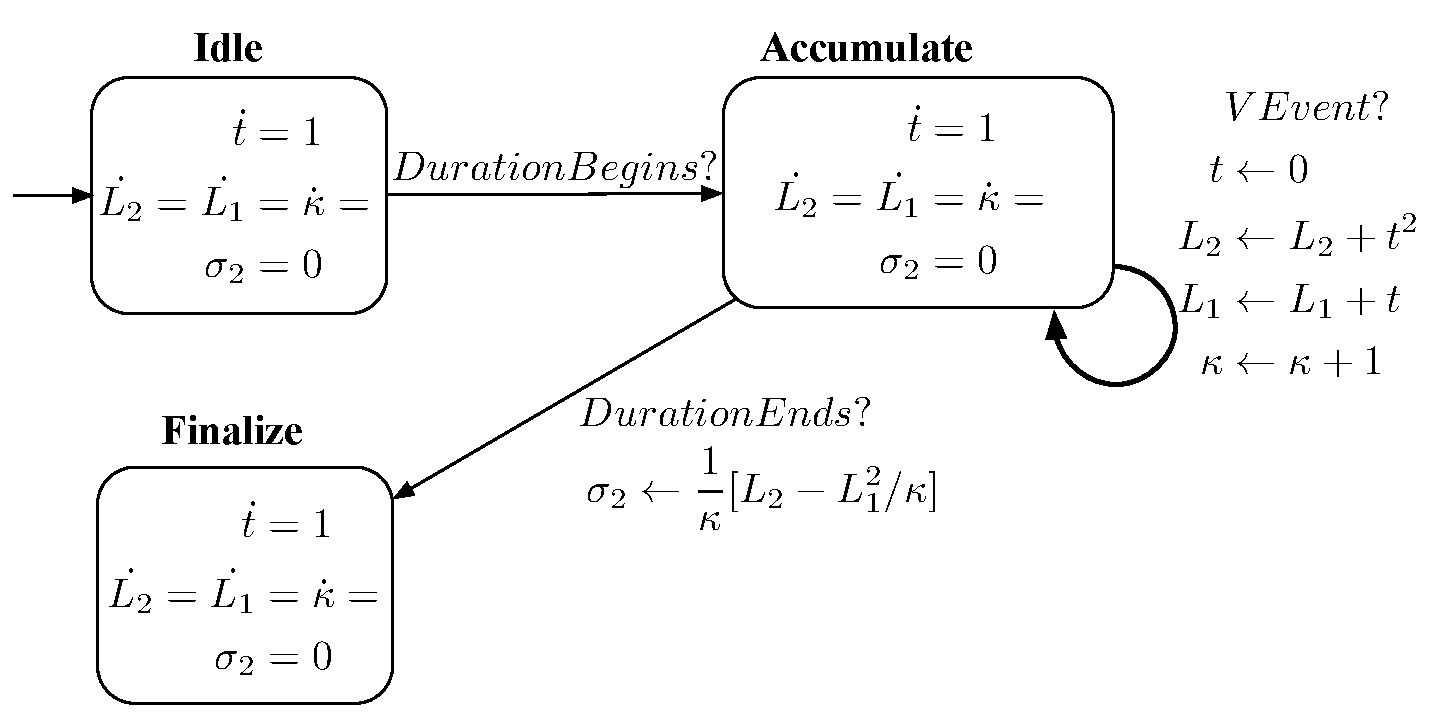
\includegraphics[scale=0.3]{figures/stability1v2}
	\vspace{-10pt}
	\caption{Stability discriminator.}
	\vspace{-10pt}
	\label{fig:Hstab}
\end{figure}

\begin{lemma}
	\label{lemma:stability}
	$\Sys_{Stab}$ is STORMED.	
\end{lemma}
The proof is in the Appendix.

Now that each system was shown to be STORMED, it remains to establish that their parallel composition is STORMED.
This result does not hold in general - Thm.~\ref{thm:SHS composition} gives conditions under which parallel composition respects the STORMED property.
Intuitively, we require that whenever a sub-collection of the systems jumps, the remaining systems that did not jump are separated from all of their respective guards by a uniform distance.
This is a requirement that can be shown to hold for our systems by modeling various minimal delays in the systems' operation. 
%For example, when a $VEvent?$ is issued by $\Sys_{Sense}$, $\Sys_{VTC}$ does not jump and will wait at least until the sampling time of the next fiducial point to make a transition.
%Or, when an atrial cell fires (in $\Sys_{CA}$), we model a minimal delay between it and all other cells that do not fire simultaneously.
We may now state:
\begin{thm}
Consider the collection of systems $\Sys_{CA}$, $\Sys_{ICD} = \Sys_{Sense} || \Sys_{Detection-Algo}$ where the latter is the parallel composition of the discriminator systems.
This collection satisfies the hypotheses of Thm. \ref{thm:SHS composition} (Section \ref{sec:compositionality}) and therefore the parallel system  $\Sys_{CA} || \Sys_{ICD}$ is STORMED and has a finite bisimulation.
\end{thm}


%\section{Properties of interest}
\label{sec:properties}
The finite simulation we obtain by running (the approximate version of) Alg.~\ref{algo:bisimulation} abstracts away the duration of continuous transitions $\trans{\tau}$, so that only time-unbounded properties (like LTL) can be verified on the abstraction.
%A priori, this is a shortcoming of the approach because many properties of interest for ICDs involve bounds on when events happen. 
However, every component of $\Sys_{ICD}$ has a local clock in its state vector.
Thus these clocks can be used to express interesting time-bounded properties of $\Sys_{ICD}||\Sys_{CA}$.

For example, to expresses that a Sustained \ac{VT} event should be followed by a \ac{VT} determination within 30sec, we write:
\begin{equation}
\label{eq:fTh}
\formula_{Th} \defeq \formula_{VT} \implies \formula_{VT} \until_{[0,30]} \Sys_{ICD}.Mode = VT
\end{equation}
The VT decision ($\Sys_{ICD}.Mode = VT$) can be reached by one of three paths of execution (see Fig. \ref{fig:bsc detection}):
For example, path $P_1$ goes from the root to ``8/10 faster'' on the right and ends in VT.
Along each path, the component automata have local clocks that keep track of how long they are running in this execution.
Therefore, the total execution time of all automata on a given path must be less than 30sec.
So the time constraint may now be expressed as the disjunction $\lor_{P \in \{P_1,P_2,P_3\}}\sum_{c\in P} c \leq 30$.
The formula can be re-written
\begin{equation*}
\formula_{VT} \implies \formula_{VT}\until \lor_{k=1,2,3}(\Sys_{ICD}.Mode = VT_k \land \sum_{c \in P_k} c \leq 30)
\end{equation*}
where $VT_k$ is the VT decision reached along the $k^{th}$ path.
%

%Letting VD denote a spontaneous (non-conducted) Ventricular Depolarization, the following formula describes a sequence of ventricular depolarizations that are 200ms or less apart.
%\begin{equation}
%\formula_{VF} \defeq VD \land \eventually_{[0,200]} (VD \land \eventually_{[0,200]} (VD \ldots))
%\end{equation}

%In terms of our model, a ventricular depolarization can be described as follows.
%Let $\Cc$ be a set of ventricular cells in the heart model that are meant to be the source of the depolarization, and let $\Nc(\Cc)$ be a neighborhood of these cells.
%The following expresses that the neighborhood is quiescent until the cells in $\Cc$ become active, implying spontaneous activity.
%Incidentally, this is a formula that does \emph{not} require time bounds, and so can be directly expressed in LTL.
%\begin{equation}
%VD \defeq \land_{c \in \Nc} (c.Mode = Quiescent) \until \land_{c\in \Cc} (c.Mode = Upstroke)
%\end{equation}
%Other ways of describing this event may be possible or preferable based on other factors.
%
%\todo[inline]{cite GF, Donze?}
%Signals used in TFL properties are also o-minimal (if the underlying time-domain signal is o-minimal), thus TFL properties can also be verified.
%Indeed, TFL properties use the Short-Time Fourier Transform (STFT) coefficients of the signal $x(t)$ to define predicates ($i=\sqrt{-1}$):
%\begin{eqnarray*}
%c_\omega(\tau) &=& \int_{\tau-L/2}^{\tau+L/2}x(t)g_L(t-\tau)e^{-i2\pi\omega t}dt
%\\
%&=& \int_{\tau-L/2}^{\tau+L/2}x(t)g_L(t-\tau)cos{2\pi\omega t}dt 
%\\
%&\quad& - i\int_{\tau-L/2}^{\tau+L/2}x(t)g_L(t-\tau)sin{2\pi\omega t}dt 
% \\
% &=& C_r(\tau+L/2) - C_r(\tau-L/2) 
% \\
% &\;& - i[C_i(\tau+L/2) - C_i(\tau - L/2)]
%\end{eqnarray*}
%Each of the summands is an integral. 
%The integrand in each is the product of a definable $x(t)$ and an analytic bounded $cos$ or $sin$ (bounded because multiplied by the window function $g_L$ of width $L$), and therefore it is definable. 
%So the antiderivatives $C_r,C_i$ are definable by a corollary of Spessegger \cite{Speissegger99_Pfaffian}.
%%($I \supset [\tau-L/2,\tau+L/2], a=\tau-L/2$), 
%So the real and imaginary parts of $c_\omega(\tau)$ are definable.
%If we identify the complex field $\Ce$ with $\Re^2$ and map the field operations of $\Ce$ to those of $\Re^2$ in the usual way, then $\Ce$ and its field operations are definable in $\Re$ and every algebraic subset of $\Ce^n$ is definable in $\Re$ \cite{PeterzilS04_ComplexOminmal}.
%Thus the function $\tau \mapsto c_\omega(\tau)$ is o-minimal being the result of applying multiplication (by $i$) and addition to definable terms.
\section{Composing STORMED systems}
\label{sec:compositionality}
The results in this section and the next apply to STORMED systems in general, including those with time-unbounded operation.
We write $[m] = \{1,\ldots,m\}$.
Given hybrid systems $\Sys_1,\ldots,\Sys_m$ in this section, $x^i, \guard^i, \theta^i,\ldots$ etc refer to a state, guard, flow $\ldots$ of system $\Sys_i$.
%
Recall that $\theta_{\ell}(t;x)$ is the flow starting at $(\ell,x)$.
The parallel composition $\Sys = \Sys_1 || \ldots ||\Sys_m$ is defined in the usual way:
$\Sys.\stSet = \Pi_i \stSet^i$,
$\Sys.\modeSet = \Pi_i \modeSet^i$,
$\Sys.\hsSet_0 =\Pi_i \hsSet_0^i$,
$Inv(\ell) = \Pi_{i}Inv^i(\ell^i)$,
$\theta_{\ell}(x,t)= [\theta_{\ell^1}^1(x^1,t),\ldots,\theta_{\ell^m}^m(x^m,t) ]^T$.
The system jumps if any of its subsystems jumps.
%, so its guard sets are of the form 
%$A^1\times\ldots \times A^m$ where for at least one $i$, $A^i$ is a guard of $\Sys_i$, and for the rest $A^j =\stSet^j$.
When a guard of a subsystem is satisfied, the state of that subsystem is reset according to its reset map.
The guards are disjoint to avoid non-determinism.
%\yhl{A system $\Sys$ is \emph{deterministic} if to every initial state $(\mode,\stPt)$, $\Sys$ produces a unique trajectory starting there.}

We show that the parallel composition of SHS is still a SHS.
In general $\Sys$ is not separable: indeed for any candidate value of $d_{min}$, one could find a transition $(i,j)$ of $\Sys$ due to, say, a jump of $\Sys_1$, s.t. at that moment $x^2$ is closer than $d_{min}$ to one of its own guards, say $\guard^2_{(j^2,k^2)}$. 
This causes $\Sys$ to further jump $j \rightarrow k$ without having traveled the requisite minimum distance, thus violating the separability of $\reset_{ij}(\guard_{ij})$ and $\guard_{jk}$.
Therefore we need to impose an extra condition on minimum separability \emph{across} sub-systems.
\begin{thm}
	\label{thm:SHS composition}		
	Let $\SHS_i = (\Sys_i, \Ac, \phi^i,b^{i,-},b ^{i,+}, d_{min}^i, \varepsilon^i, \zeta^i)$, $i=1,\ldots,m$ be deterministic SHS 
	defined using the same underlying o-minimal structure, 
	and where each state space $\stSet^i$ is bounded by $B_{X^i}$.
	\\
	Define parallel composition $\SHS = (\Sys, \Ac, \phi,b^-,b^+, d_{min}, \varepsilon, \zeta)$ where
	$\Sys = \Sys_1 || \ldots ||\Sys_m$,	
	$\phi = (\phi^1,\ldots,\phi^m)^T \in \Re^{mn}$,
	$b^{i,-} = \inf_{x \in \stSet} \phi\cdot x$,
	$b^{i,+} = \sup_{x \in \stSet} \phi\cdot x$,
	$\varepsilon = \min(\min_i \varepsilon^i, \min_i \frac{\zeta^i}{B_{X^i}})$,
	$\zeta = \min_i \zeta^i$ and
	\[d_{min} = \min_{I\subset [m]} (\min_{i\in I}d_{min}^i, \min_{i\in I ,j \in [m]\setminus I }d_{min}^{ij})\]	
	Assume that the following \textbf{Collection Separability} condition holds: 	
	\yhl{for all $i,j \leq m, \neq j $ there exists $d_{min}^{ij}>0$ s.t. 
		\yhl{if $\stPt \in \stSet$ is in the reachable set of $\Sys$} and 
		$x^i \in G^i_e \land x^j \notin G^j_{e'} \; \forall e' \in E^j$ 
		then $d(x^j,G^j_{e'}))>d_{min}^{ij}$ for all $e'\in E^j$ 
		where $E^j$ is the edge set of $\SHS_j$ and $G^j_{e'}$ is a guard of $\SHS_j$ on edge $e' \in E^j$.}
	Then $\SHS$ is STORMED.
\end{thm}

\section{Finite simulation for STORMED systems}
\label{sec:simulationAprox}
In general it is not possible to compute the reach sets required by the iteration \eqref{eq:Ft,Fd} exactly unless the underlying theory is decidable.
The $\Sys_{ICD}||\Sys_{CA}$ closed loop is definable in $\Lc_{\exp}$, and the latter is not known to be decidable.
%The authors in \cite{PrabhakarVVD09_toklerant} proposed approximating the flows and resets by polynomial flows and resets in the decidable theory $\Lc_\Re$.
%However, the approximation process is typically iterative and requires manual intervention, or is restricted to subclasses of STORMED systems \cite{PrabhakarVVD09_toklerant}.
Here we show that if an approximate reachability tool with definable over-approximations is available for the continuous dynamics, it can be used in \eqref{eq:Ft,Fd} to yield a finite \emph{simulation}.
Since we only have a simulation, counter-examples on the abstraction should be validated in a CEGAR-like fashion.
\begin{lemma}
	\label{lemma:finite simu}
	Let $\SHS = (\Sys,\ldots)$ be a SHS and $\sim$ an equivalence relation on $\stSet$.
	For any mode $\mode$ of $\Sys$, the dynamical system $\Dc$ with state space $X = \Sys.\stSet$ and set-valued flow $\Theta(t;x) = \{y \in \Re^n \;|\; ||y-\theta(t;x)||^2 \leq \epsilon^2\}$ admits a finite simulation $\simu_\mode$ that respects $\sim$.
\end{lemma}
Let $\Ft^\epsilon(\partition) \defeq \cap_{\mode}\simu_{\mode \in \modeSet}$ where $\partition = \stSet/\sim$. $\Ft^\varepsilon$ refines all the $\simu_\mode$'s, and it is a finite simulation of $\Sys$ by itself w.r.t. the continuous transition $\trans{\tau}$.

\begin{thm}
	\label{thm:finite simulation}
	Let $\Sys$ be a STORMED hybrid system, 
	and $\partition$ be a finite definable partition of its state space.
	Define 
	\begin{equation}
	\label{eq:Fte,Fde}
W_0 = \Ft^\epsilon(\partition), \quad \forall i\geq 0, W_{i+1} = \Ft^\epsilon(\Fd(W_i))
	\end{equation}
Then there exists $U \in \Ne$ s.t. $W_{U+1} = W_U$ and $\Ft^\epsilon(W_U)$ is a simulation of $\Sys$ by itself.
\end{thm}

\section{Conclusion}
In this paper, we presented the first formalization of a hybrid system model of the human heart and the \ac{ICD} device and showed that the resulting closed-loop may be formally verified. 
We showed that the heart model, the \ac{ICD} measurement process, the modules of common \ac{ICD}, and the parallel composition of the entire system to be a STORMED hybrid system, which admits finite bisimulation.
In the process, we were able to show that approximate reachability yields finite simulation for STORMED systems and that certain composition respect the STORMED property.
Finally, we showed that the reach set computed by SpaceEx may be used to build the simulation.


\bibliographystyle{abbrv}
\bibliography{HSCC2015_CompositionalConf,houssam,fainekos_bibrefs,hscc2016,biblio2}  %zhihao
% ACM needs 'a single self-contained file'!
%
%\clearpage
\appendix
%
%vtcextension
% tfl
\subsection{Transition and hybrid systems}
\label{sec:transition systems}

%{\large Partitions.} Given a set $Q$, a \emph{partition} $\partition = \{P_1,\ldots,P_k\}$ of $Q$ is a set of disjoint subsets of $Q$ whose union equals $Q$. 
%Let $\equiv_\partition$ be the associated equivalence relation.
%Partition $\partition'$ \emph{refines} $\partition$ if every block $P'$ of $\partition'$ is a subset of some block $P$ of $\partition$; we write this as $\partition' \subset \partition$.
%
\begin{defn}
	\label{defn:transition system}
	A \emph{transition system} $T = (Q,\labelSet,\trans{},Q_0)$ consists of a set of states $Q$, a set of events $\labelSet$ , a transition relation $\trans{} \subset Q \times \labelSet \times Q$, a set of initial states $Q_0$. 
	We write $q \trans{\slabel}q'$ to denote a transition element $(q,\slabel,q') \in \trans{}$.
	Given $P\subset Q$, we define $Post_\slabel(P) \defeq \{q'\;|\;\exists q\in P. q \trans{\slabel}q'\}$
	%
	Given an equivalence relation $\sim$ on $Q$, the \emph{quotient system} $T/\sim$ is
	$T/\sim = (Q/\sim, \{*\}, \trans{}_\sim, Q_0/\sim)$
	where $[q] \trans{*}_\sim [q']$ iff $q \trans{\slabel} q'$ for some $\slabel \in \labelSet$.
	Here $[q]$ is the equivalence class of $q$ and $Q/\sim$ is the set of equivalence classes of $\sim$.
\end{defn}

\begin{defn}
	\label{defn:simulation}	
	Given two transition systems $T_1$ and $T_2$ with the same state space $Q$,
	a \emph{simulation} relation from $T_1$ to $T_2$ is a relation $\simu \subset Q \times Q$ such that 
	for all $(q_1,q_2) \in \simu$, if $q_1 \trans{\slabel}_1 q_1'$, there exists a $q_2' \in Q$ s.t. $q_2 \trans{\slabel}_2 q_2'$ and $(q_1',q_2') \in \simu$.
	A \emph{bisimulation relation} between $T_1$ and $T_2$ is both a simulation relation from $T_1$ to $T_2$ and from $T_2$ to $T_1$.
\end{defn}
%Given a partition $\partition$ of $Q$, the \emph{natural bisimulation} between $T$ and $T/\partition$ is $\Bc_P = \{(q,P) \in Q \times \partition \;|\; q \in P\}$.	
%Conversely, a bisimulation $\Bc$  of $T$ defines a partition $\partition_\Bc$ of $Q$ where $q,q'$ are in the same block of the partition iff $(q,q') \in \Bc$.
%
The bisimulation $\bisimu$ is said to \emph{respect} $\sim$ if $(q,q') \in \bisimu \implies q \sim q'$.
%
The following algorithm, if it terminates, yields a finite bisimulation for $T$ that respects the given equivalence relation~\cite{AlurHLP00ieee}.
Moreover, it is the \emph{coarsest} bisimulation (with respect to inclusion) that respects $\sim$.
\begin{algorithm}[t]
		\caption{Computing a bismimulation respecting $\sim$}
		\label{algo:bisimulation}
		\begin{algorithmic}
			\Require Transition system $T = (Q,\labelSet,\trans{},Q_0)$, equivalence relation $\sim$.
			\State Set $\simu = Q/\sim$			
			\While{$\exists P,P' \in \simu$ and $\slabel \in \labelSet$ s.t. $\emptyset \neq P' \cap Post_\slabel(P) \neq P'$}
				\State Set $\simu = \simu \setminus \{P'\} \cup \{P' \cap Post_\slabel(P) , P' \setminus Post_\slabel(P) \}$
			\EndWhile	
			\State Return $\simu$
		\end{algorithmic}
\end{algorithm}
Given a set of atomic propositions $AP$, if $\sim$ is s.t. $q \sim q'$ iff both states satisfy exactly the same set of atomic propositions, then model checking temporal logic properties can be done on the finite bisimulation instead of the possibly infinite $T$.
%The \emph{coarsest} bisimulation $\bisimu$ that refines a partition $\partition$ is one such that there is no other bisimulation $\bisimu'$ satisfying $\partition_\bisimu \subset \partition_{\bisimu'} \subset \partition$.

%Given a subset $P$ of $Q$, we define its $\slabel$-successor as $Post_\slabel(P) = \{q \in Q | \exists p \in P. q \trans{\slabel} p\}$.
%In other words, $Post_\slabel(P)$ is the set of states forward-reachable from $P$ via the event $\slabel$.


%
%Note that the resulting bisimulation is the \emph{coarsest} bisimulation (i.e., with the least number of blocks in its induced partition) that refines $\partition$.
{\large \textbf{Ends Delimited}}
We need the following result in what follows.
\begin{prop}
	\label{prop:ED}
	If the state space $\stSet$ of a hybrid automaton $\Sys$ is bounded, then its guards have delimited ends.
\end{prop}
\begin{prf}
	For all guard sets $G$ and all $x \in G$, $||\phi \cdot x || \leq ||\phi|| \cdot ||x|| \leq ||\phi||.\max\{||x||, x\in \stSet \} < \infty$.
\end{prf}
\input{proofHeartCA}
\input{proofSensing}
\subsection{Three Consecutive Fast Intervals}
\label{sec:tcfi}
\begin{figure}[t]
	\centering
	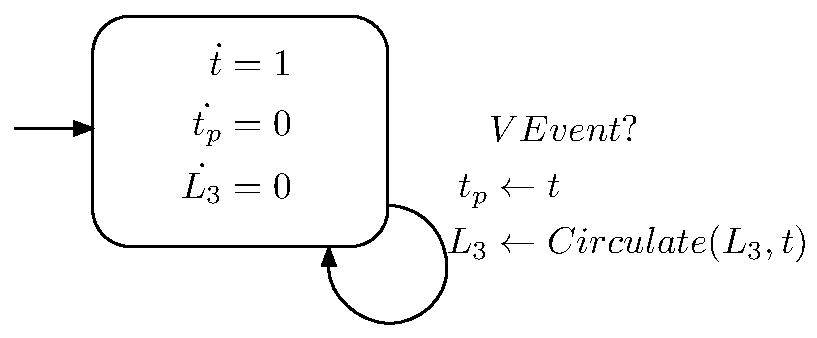
\includegraphics[scale=0.3]{figures/TCFI}
		\vspace{-10pt}
	\caption{Three Consecutive Fast Intervals $\Sys_{TCFI}$}
	\label{fig:tcfi}
\end{figure}
Our first module simply detects whether three consecutive fast intervals have occurred, where `fast' means the interval length, measured between 2 consecutive peaks on the \ac{EGM} signal, is shorter than some pre-set amount.
See Fig. \ref{fig:tcfi}.
States $t$ and $t_p$ are clocks as before.
The vector $L_3$ is three-dimensional, and stores the values of the last three intervals.
The event VEvent? is shorthand for the transition $y(t) \geq Th$ being taken by the $\Sys_{Sense}$ automaton.
In other words, it indicates a ventricular event.
Then $L_3$ gets reset to $L_3^+ = (z_1,z_2,z_3)^+ \defeq \text{Circulate}(L_3,t-t_p)$ where
\begin{equation}
L_3^+ = 
\left(\begin{matrix}
z_2\\z_3\\t-t_{p}\\
\end{matrix}
\right)
=
\left(\begin{matrix}
0 & 1 & 0\\0& 0& 1\\0& 0 &0
\end{matrix}
\right) L_3 + 
\left(\begin{matrix}
0\\0\\t-t_p
\end{matrix}
\right)
\end{equation}
%
\begin{lemma}
	$\Sys_{TCFI}$ is STORMED.
\end{lemma}

{\large \textbf{Proof of Lemma \ref{lemma:vtc}.}}
\begin{prf}
\textbf{S}eparability obtains by observing that a uniform minimum time passes between beats and between samples. 
\textbf{T}ISG is immediate.
\textbf{O}-minimality is established by observing that all sets and functions are definable in $\Lc_{\exp}$. \textbf{ED} holds because the state space is bounded.
We now show monotonicity.
The state of the system is $x = (t , \mu ,\alpha, \beta , \vec{\nu}, w)^T \in \Re^{4+10+1}$.
Let $\phi = (\phi_c,\phi_\mu,\phi_\alpha,\phi_\beta,\phi_1,\ldots,\phi_{10},\phi_w)^T \in \Re^{15}$ be the corresponding vector.
For flows in mode CalculateVTC, we seek a $\phi$ and $\varepsilon > 0$ such that 
$\phi \cdot (t+\tau -  t , \mathbf{0} , -\gamma(t+\tau) + \gamma t) = \phi_c \tau + \phi_w(-\gamma \tau) \geq \varepsilon \sqrt{\tau^2 + \gamma^2\tau^2}$,
which is equivalent to 
$\boxed{\phi_c - \phi_w\gamma \geq \varepsilon \sqrt{1 + \gamma^2}}$.
Reset monotonicity for resets R1, R2, R3 provides three more constraints on $\phi$ and $\varepsilon$:
\begin{eqnarray*}
&\mathbf{(R1)} &
\phi \cdot (-t, -\mu , -\alpha , -\beta ,\nu_2 - \nu_1 , \nu_3 - \nu_2 , \ldots , -1 - \nu_{10}, \yhl{1-w})
\\	
&=& -\phi_c t -\phi_\mu \mu -\phi_\alpha \alpha - \phi_\beta \beta + \sum_{i=1}^{10}\phi_i(\nu_{i+1}-\nu_i) 
\\
&&+ \phi_w(1-w) \stackrel{Want}{\geq} \zeta
%
%
\\
%
%
&\mathbf{(R2)} &
\phi \cdot (t-t , \egm , \egm \egm_m, \egm^2 , \mathbf{0} , 1-w)
\\
&=& \phi_\mu \egm + \phi_\alpha \egm \egm_m+ \phi_\beta \egm^2 + \phi_w (1-w) \stackrel{Want}{\geq} \zeta
%
%
\\ 
&\mathbf{(R3)} &
 -\phi_c t -\phi_\mu \mu -\phi_\alpha \alpha - \phi_\beta \beta + \sum_{i=1}^{10}\phi_i (\nu_{i+1}-\nu_i) 
 \\
 && + \phi_w(1-w) \stackrel{Want}{\geq} \zeta
\end{eqnarray*}
where $\nu_{11} \defeq -1$ in $\mathbf{R1}$ and $\nu_{11}\defeq 1$ in $\mathbf{R3}$.
%
Combine $\mathbf{R1}$ and $\mathbf{R3}$ by choosing $\phi_1 = \ldots = \phi_{10}=\phi_\mu = \phi_\alpha = \phi_\beta = 0$:
\begin{eqnarray*}
\label{eq:R23}
\mathbf{(R1,3)}\; -\phi_c t + \phi_w(1-w) \geq \zeta
\\
\mathbf{(R2)}\; \phi_w(1-w) \geq \zeta
\end{eqnarray*}
Now note that when a reset occurs, $0<w \leq 1-\gamma T_s \defeq w_m$ where $T_s$ is the smallest sampling period, and that $t\leq 10B$, $B$ = the maximum peak-to-peak interval, so $\mathbf{(R2)} ,\mathbf{(R1,3)} $ can be jointly satisfied if $\boxed{-\phi_c10B + \phi_w(1-w_m) \geq \zeta}$.
The 2 boxed equations can be jointly satisfied.
	\end{prf}
Proof of Lemma \ref{lemma:stability}.
\begin{prf}
We show the resets are monotonic - the other properties are immediate.
The state is $x = (t,L_2,L_1,\kappa,\sigma_2)^T$.
The self-transition ACCUMULATE $\rightarrow$ ACCUMULATE is initiated by VEvent (ventricular peak).
At reset time, $0 \leq t \leq DL$, we have that 
$\phi\cdot(0-t,t^2,t,1,0)^T \geq -\phi_1 DL + \phi_4 \stackrel{Want}{\geq} \zeta$.

The transition ACCUMULATE $\rightarrow$ FINALIZE, initiated at the end of Duration, saves the value of the variance in $\sigma_2$.
This reset produces the constraint
$\phi_5 ((L_2 -L_1^2/\kappa)/\kappa) \geq \varepsilon |((L_2 -L_1^2/\kappa)/\kappa)|$.
But the quantity in absolute value is itself a variance and so is positive, therefore the constraint is simply $\phi_5 \geq \varepsilon$, compatible with the previous inequality.
\end{prf}
\yhl{{\large \textbf{An equivalent characterization of Collection Separability}.}
	\\
Collection separability (Thm. \ref{thm:SHS composition}) can be equivalently expressed in terms of set operations. 
Let $R$ be the reachable set of $\Sys$,
and let $R_{|ij}$ be the projection of $R$ onto the space $\stSet^i \times \stSet^j$.
Then Collection Separability is expressed as:
\\
for all $i,j \leq m, i\neq j$ there exists $d_{min}^{ij}>0$ s.t. for all guards $\guard^i$ of $\Sys_i$ and all guards $\guard^j$ of $\Sys_j$, \begin{equation*}
R_{|ij} \cap \guard^i \times (\stSet^j \setminus \guard^j) \subset \stSet^i \times \{x^2 \in \stSet^2 \;|\; d(x^2,\guard^2) > d_{min}^{ij}\}
\end{equation*}}
\input{proofSHSComposition}
Proof of Lemma \ref{lemma:finite simu}.
\begin{prf}
	This follows the lines of the elegant proof of \cite{BrihayeM05_ominimal} as formulated in \cite{tabuada} and generalizes it to set-valued maps.
	(The fact that using an approximate $Post$ operator yields a simulation is a special case of a more general result on transition systems but we prove it here for completeness).
	
	First observe that using approximate reachability on a system $\Sys$ is tantamount to replacing $\Sys$ with a system $\Sys^\varepsilon$ whose flows and reset maps are set-valued $\varepsilon$ over-approximations of the flows and resets of $\Sys$ (but is otherwise unchanged).
	Therefore define the dynamical system $\Dc^\varepsilon$ with state space $\stSet$ and whose flow $\Theta: \Re \times \Re^n \rightarrow 2^{\Re^n}$ is a set-valued $\varepsilon$ over-approximation of $\theta_\mode$:
	$\Theta(t;x) = \{y \in \Re^n \;|\; ||y-\theta(t;x)||^2 \leq \epsilon^2\}$.	
	Let $\partition \defeq \stSet/\sim$ be the partition induced by $\sim$.
	%
	It follows from the definability of $\theta$ and $||\cdot||^2$ that $\Theta$ is definable. 
	Given $P \in \partition$, let $Z(P) = \Theta^{-1}(P) \defeq \{(x,t) \;|\; \Theta(x,t) \cap P \neq \emptyset\}$.
	Then $Z(P)$ is definable because $P$ and $\Theta$ are definable.
	Let $Z_x(P) = \{t \;|\; (x,t) \in Z(P)\} \subset \Re$ be the \emph{fiber} of $Z$ over $x$.
	The number of connected components of $Z_x(P)$ equals the number of times that $\Theta(x,t)$ intersects $P$.
	Now it follows from \cite{tabuada} Thm.7.11 that there exists a uniform upper bound on the number of connected components of $Z_x(P)$, independent of $x$.
	Let that bound be $V_P$.
	Thus $\Theta(x,t)$ visits $P$ at the most $V_P$ times, regardless of $x$.
	Since there is a finite number of blocks $P \in \partition$, then $\Theta(x,t)$ visits any block $P$ a maximum of $V \defeq \max_P(V_P)$ times.%, independent of $x$ and $P$.
	
	Thus we can associate to each $x\in \stSet$ a finite number of finite strings $q(x) = (\ell_1,\ell_2,\ldots,\ell_{i-1},\widehat{\ell_i},\ell_{i+1},\ldots,\ell_s)$, where $\ell_i,\widehat{\ell}_i \in \partition$.
	Each $q(x)$ gives the sequence of blocks that $\Theta(x,t)$ visits (with repetition), and in which $\widehat{\ell_i}$ is the block containing $x$.
	There may be more than one such string because the set $\Theta(x,t)$ might intersect more than one block of $\partition$ at a time.		
	The length of $q(x)$ is thus uniformly upper-bounded by $V\cdot |\partition|$, so there's a finite number of different strings $q(x)$. 
	%
	Let $\Qc(x)$ be the set of such strings associated to $x$, and let $\Qc = \cup_x \Qc(x)$.
	Then $\Qc$ is the state space of the finite transition system $K = (\Qc,\{*\},\trans{},\Qc_0)$ whose transition relation is 
	\begin{compactitem}
		\item $\ell_1\ldots\widehat{\ell}_i\ldots\ell_s \trans{*} \ell_1\ldots\widehat{\ell}_{i+1}\ldots\ell_s$
		\item $\ell_1\ldots\ell_{s-1} \widehat{\ell_s} \trans{*} \ell_1\ldots\ell_{s-1} \widehat{\ell}_s$
	\end{compactitem}

	It is clear that $K$ is non-deterministic and simulates $\Dc$ but is not a bisimulation because of the over-approximation produced by $\Theta$.	 
\end{prf} 
{\large \textbf{Proof of Theorem \ref{thm:finite simulation}.}}
\begin{prf}
	First observe that $\Ft^\epsilon(\cdot)$ is idempotent: $\Ft^\epsilon(\Ft^\epsilon(\partition)) = \Ft^\epsilon(\partition)$.
	
By Lemma 10 of \cite{VladimerouPVD08_STORMED} there exists a uniform bound $U$ on the number of discrete transitions of any execution of the STORMED system $\Sys$, so $\Fd(W_k) = W_k$ for all $k\geq U$.
Moreover 
$W_{U+1} = \Ft^\epsilon(\Fc_d(W_U)) = \Ft^\epsilon(W_U)$
and $W_{U+2}= \Ft^\epsilon(\Fc_d(W_{U+1}))= \Ft^\epsilon(W_{U+1})= \Ft^\epsilon(\Ft^\epsilon(W_U)) = \Ft^\epsilon(W_U) = W_{U+1}$, so the iterations reach a fixed point.
The fact that $\Ft^\epsilon(W_U)$ is a simulation then yields the desired result.
\end{prf}
\subsection{Example: SpaceEx reachable sets}
\label{sec:spaceex}
Lemma \ref{thm:finite simulation} required that the over-approximation sets $\Rc^\epsilon_{t}(\{{x}\})$ be definable for every $x$ and $t$ (see proof).
In practice, we need to show that the over-approximation \emph{actually computed by the reachability tool} (which may not be the full ball $\Rc^\epsilon_{t}(x)$) is definable.
In this section we show that the over-approximations computed by SpaceEx \cite{FrehseCAV11} are definable.
Given the set $X\subset \Re^n$ and finite $\Vc \subset \Re^n$, parameter $\lambda \in [0,1]$ a time step $\delta>0$, and $(i,j) \in E$, 
SpaceEx over-approximates $\reset_{ij}(X)$ by $\Kc(\Vc,X) \defeq \reset_{ij}(TH_\Vc(X)\cap G_{ij})\cap Inv(j)$ and $\Rc_{\lambda \delta}^\epsilon(X)$ by \cite{FrehseCAV11}:
\begin{eqnarray}
\Omega_\lambda(X,\delta) &=& (1-\lambda)X \oplus e^{\delta A} X 
\nonumber \\
&\oplus&(\lambda E_\Omega^+(X,\delta) \cap (1-\lambda) E_\Omega^-(X,\delta))
\end{eqnarray}
where
$TH_\Vc(X) \defeq \{x\in\Re^n \;|\;\land_{\vec{a} \in \Vc} \vec{a}\cdot x \leq \rho(\vec{a},X)\}$ is the template hull of $X$ and $\rho$ its support function,
$E_\Omega^+ = \boxdot (\Phi_2 \boxdot(A^2 X)$,
$E_\Omega^- = \boxdot (\Phi_2 \boxdot(A^2 e^{\delta A}X))$,
$\oplus$ is the Minkowski sum,
$\boxdot S =  [-\overline{|x_1|}, \overline{|x_1|} ] \times \ldots \times [-\overline{|x_n|}, \overline{|x_n|} ]$ is the box hull
with $\overline{|x_i|} \defeq \max\{|x_i| \text{ s.t. } x=(x_1,\ldots,x_n) \in S\}$.

\begin{thm}
	\label{thm:spaceex definable}
	For all definable polytopes $X \subset \Re^n$, the sets $\Kc(\Vc,X)$ and $\Omega_\lambda(X,\delta)$ is definable are $\Lc_{\exp}$.
\end{thm}
	
\begin{prf}
Let $S, Y \subset \Re^n$ be two definable sets in some o-minimal structure $\Ac$.
Let $\lambda \in \Re$ and let $A$ be a real matrix.
Then the following sets are also o-minimal: $\lambda S$, $A S$, $S \cap Y$, $S \oplus Y$, $S \cap Y$, $TH_\Vc(S)$ and $\boxdot S$.
Now the result follows by noting that $\Kc(\Vc,X)$ and $\Omega_\lambda(X,\delta)$ are constructed by composing the above definability-preserving operations.
\end{prf}


Proof of Prop.~\ref{prop:spaceex definable}.
\begin{prf}
	\newcommand{\EPS}{\mathcal{E}}
	We show that if $S \subset \Re^n$ is o-minimal, then $\boxdot S$ and $TH_\Vc(S)$ are o-minimal. 
	O-minimality of the other sets is a standard result.
	
	We start with $\boxdot S$.
	\begin{eqnarray*}
		\boxdot S &=& \{y \in \Re^n \;|\; -\overline{|x_i|}\leq y_i \leq \overline{|x_i|},i=1,\ldots,n\}
		\\
		&=& \{y \in \Re^n \;|\; \exists a_i \in \Re_+. (a_i = \sup \{|x_i|,x\in S\} 
		\\
		&& \land (-a_i\leq y_i \leq a_i)),i=1,\ldots,n\}
		\\
		&=&  \{y \in \Re^n \;|\; \exists a_i \in \Re_+. (\forall \varepsilon_i>0 \exists x_i \in S . a_i-\varepsilon < |x_i(i)|)
		\\
		&& \land (-a_i\leq y_i \leq a_i)),i=1,\ldots,n\}
		\\
		&=&  \{y \in \Re^n \;|\; \exists a_i \in \Re_+. (\forall \varepsilon_i>0 \exists x_i \in S . a_i-\varepsilon < x_i(i)
		\\
		&& \lor a_i - \varepsilon > -x_i(i)) \land (-a_i\leq y_i \leq a_i)),i=1,\ldots,n\}
\end{eqnarray*}

The template hull is given by
\[TH_\Vc(X) \defeq \{x\in\Re^n \;|\;\land_{a \in \Vc} a\cdot x \leq \rho(a,X)\}\]
where the support function is given by 
\begin{equation}
\label{eq:supportfnt}
\rho(a,S) \defeq \max_{x \in S} a\cdot x
\end{equation}
Therefore $TH_\Vc(X)$ is definable if $\rho$ is.
The graph of $a \mapsto \rho(a,S)$ is given by 
\begin{eqnarray}
\textbf{Gph}\rho = \{(a,r) \;|\; \forall x\in S.\; r\geq a\cdot x \land \exists x\in S. r=a\cdot s\}
\end{eqnarray}
which is a first-order formula on predicates that use $+,\times$.
Since $S$ is o-minimal, Gph$\rho$ is o-minimal.
%
%To do so we show that it can be computed using a finite number of operations from the o-minimal structure $\Lc_{\exp}$.
%As we assume that $S$ is a polytope (a closed bounded intersection of half-spaces), it has a finite number of extreme points. 
%Let $\mathcal{E} =  \{e_i,i=1,\ldots,k\}$ be the set of extreme points and any point $x\in S$ can be written as a convex combination of the extreme points: $x = \sum_{i}\alpha_i e_i$.
%Therefore we can write
%\[ \rho(a,S) = \max_{\alpha \in I^k} \sum_{i=1}^k \alpha_i a\cdot e_i \]
%where $I^k = \{(\alpha_1,\ldots,\alpha_k)\;|\; \alpha_i \geq 0, \sum \alpha_i = 1\}$
%
%The maximizer $x^*$ of \eqref{eq:supportfnt} is necessarily a boundary point of $S$.
%Indeed let $x^0$ be an interior point of $S$ ($x^0 \in S\setminus \partial S$).
%Then the line through $x^0$ intersects $\partial S$ twice, at points $\lambda_1x^0$ and $\lambda_2x^0$, with $\lambda_1 \geq 1$ and $\lambda_2 \leq 1$.
%This is the case because $S$ is closed and bounded.
%If $a\cdot x^0 \geq 0$, then $a\cdot \lambda_1 x^0 \geq a\cdot x^0$. 
%And if $a\cdot x^0<0$ then $0 \geq a\cdot \lambda_2 x^0 \geq a\cdot x^0$. 
%Thus to any interior point of $S$ there exists a boundary point with a larger projection on $a$.
%
%A boundary point can always be written as the convex combination of exactly $n$ extreme points, namely the extreme points that are the vertices of the face to which the boundary point belongs.
%
%Therefore the support function expression is further simplified to:
%\[ \rho(a,S) = \max_{\alpha \in [0,1], \mathcal{F} \subset \EPS:|\mathcal{F}|=n } \sum_{i=1}^n \alpha_i a\cdot e_i \]
	\end{prf}


\end{document}
